\documentclass[12pt]{article}

\usepackage{sbc-template}
\usepackage{graphicx,url}
\usepackage{amsmath}
\usepackage[utf8]{inputenc}
\usepackage[brazil]{babel}
\usepackage{array}
\newcolumntype{L}[1]{>{\raggedright\arraybackslash}p{#1}}

\sloppy

\title{Desenvolvimento de uma Ferramenta de Modelagem Preditiva para
  Identificação de Sexo e Estimativa de Peso em Galinhas}

\author{João Vitor Santana Lima\inst{1}}

\address{Programa de Iniciação Científica ICV/UFPI\\
  Universidade Federal do Piauí (UFPI)\\
  Orientadora: Alcilene Dalília de Sousa
  \email{j.v.s.l2009@gmail.com}
}

\begin{document}

\maketitle

\section{Introdução}

Com o crescimento da avicultura e a busca por maior eficiência nos sistemas de
criação, torna-se cada vez mais necessário adotar ferramentas tecnológicas que
auxiliem no manejo das aves. A obtenção rápida, prática e confiável de
informações essenciais sobre cada indivíduo, como peso corporal e sexo,
contribui para um controle mais preciso do plantel e para a melhoria dos
índices produtivos.

A galinha-d'angola (\textit{Numida meleagris}), pertencente à ordem dos
\textit{Galliformes} e à família \textit{Numididae}, é uma ave originária da
África e foi introduzida no Brasil pelos colonizadores portugueses,
provenientes da África Ocidental. No país, também é conhecida popularmente como
guiné, galinha-do-mato, capote, capota, pintada, picote (na Amazônia) ou
tô-fraca (TARGINO, 2015). Trata-se de uma espécie rústica, com boa
adaptabilidade a diferentes condições climáticas, o que a torna relevante para
a avicultura familiar e de pequena escala em diversas regiões brasileiras
(OGAH et al., 2022).

Apesar de sua importância, a criação de galinhas-d'angola ainda carece de
tecnologias voltadas ao manejo produtivo. Nas fases iniciais de
desenvolvimento, essas aves apresentam grande semelhança morfológica entre
machos e fêmeas, o que dificulta a identificação do sexo por meio da observação
visual. Estima-se que pelo menos metade das espécies de aves existentes no
mundo não possua dimorfismo sexual evidente, sendo essa diferenciação
geralmente sutil e manifestada somente a partir da maturidade sexual (VIEIRA et
al., 2009). No caso específico da galinha-d'angola, a diferenciação entre os
sexos pode ser feita pela vocalização, onde as fêmeas emitem o característico
som ``tô-fraco'', enquanto os machos produzem arrulhos e cacarejos (BOTTINO et
al., 2006). Essa limitação compromete decisões de manejo, como a formação de
lotes, a seleção de reprodutores e o direcionamento adequado da produção.

Nesse contexto, o uso de técnicas de inteligência artificial, como as redes
neurais artificiais, surge como uma alternativa promissora para a predição do
peso corporal e a identificação do sexo de galinhas-d'angola a partir de
medidas biométricas. Na avicultura, as redes neurais artificiais já
demonstraram elevada capacidade na predição de parâmetros de desempenho
produtivo, superando modelos estatísticos convencionais na modelagem de
relações não lineares entre variáveis (SALLE et al., 2001). Esses modelos
possibilitam estimativas mais precisas e ágeis em comparação aos métodos
tradicionais, reduzem a subjetividade inerente às avaliações visuais e
favorecem a tomada de decisões em fases precoces do desenvolvimento das aves.

Apesar da relevância da espécie, ainda não existem modelos robustos que
permitam simultaneamente a predição de peso e classificação de sexo em
galinhas-d'angola a partir de medidas morfométricas. Diante do exposto, o
presente trabalho tem como objetivo desenvolver e avaliar modelos de
aprendizagem de máquina para predição do peso corporal e classificação do sexo
de galinhas-d'angola a partir de suas medidas corporais.

\section{Revisão de Literatura}

A predição de características produtivas a partir de medidas corporais em aves e
outras espécies de interesse zootécnico tem sido amplamente investigada nas
últimas décadas. Com o avanço das técnicas de inteligência artificial e
aprendizado de máquina, novos métodos vêm sendo propostos como alternativas aos
modelos estatísticos tradicionais, oferecendo maior capacidade de captura de
relações não lineares entre variáveis morfométricas e características de
interesse econômico. A presente revisão reúne os principais estudos que
fundamentam esta pesquisa, abrangendo trabalhos sobre a galinha-d'angola,
predição de peso corporal em aves e outras espécies, e a aplicação de
diferentes técnicas computacionais na modelagem preditiva.

(OGAH et al., 2012) avaliou a relação entre medidas corporais e características
de carcaça em galinhas-d'angola indígenas da Nigéria, utilizando 28 aves
adultas de ambos os sexos. Os resultados mostraram que o perímetro torácico foi
o melhor preditor isolado do peso corporal (R² = 0,558), enquanto o peso
corporal destacou-se como a variável mais importante na predição do peso de
carcaça (R² = 0,820) e do peso do peito (R² = 0,902). O estudo demonstra que
medidas lineares simples podem ser utilizadas com razoável precisão para
estimar o peso vivo e características de carcaça em galinhas-d'angola.

(DZUNGWE et al., 2018) investigaram a relação entre peso corporal e medidas
lineares em galinhas-d'angola francesas de corte, criadas em condições
tropicais úmidas na Nigéria. Um total de 86 aves foi avaliado com 38 semanas de
idade, mensurando-se comprimento da canela, comprimento da coxa, comprimento da
quilha, perímetro torácico, comprimento corporal e comprimento da asa. As
correlações entre peso corporal e medidas lineares foram positivas e
significativas (P < 0,01). O comprimento da canela apresentou o maior
coeficiente de determinação (R2 = 19,5\%), indicando ser o melhor preditor do
peso corporal nessa linhagem.

(PORTILLO-SALGADO et al., 2021) utilizaram regressão linear múltipla e análise
de árvore de regressão (algoritmo CHAID) para predizer o peso de ovos de
galinhas-d'angola a partir de características externas. Foram avaliados 110 ovos
de um lote com 23 semanas de idade. A área de superfície do ovo foi a variável
preditora mais importante, explicando 72\% da variação no peso do ovo por
regressão linear e 74\% pela árvore de regressão. Ambos os métodos estatísticos
demonstraram precisão semelhante, confirmando que características externas dos
ovos podem ser utilizadas de forma confiável para estimar seu peso.

(REIS et al., 2008) estudaram a predição do peso vivo a partir de medidas
corporais em bovinos mestiços Holandês/Gir, utilizando dados de 483 vacas, 469
novilhas e 62 machos. Embora o estudo tenha sido conduzido com bovinos, a
abordagem metodológica é relevante para o presente trabalho. O perímetro
torácico apresentou a maior correlação com o peso corporal em todas as
categorias (0,807 para vacas; 0,928 para machos; 0,942 para novilhas). Modelos
polinomiais cúbicos proporcionam alta aderência, demonstrando que uma única
medida corporal pode ser suficiente para estimativas precisas do peso.

(JAHAN et al., 2020) desenvolveram um modelo de rede neural artificial (RNA) do
tipo perceptron multicamadas para predizer o peso de abate de codornas
japonesas com base no desempenho de crescimento inicial, sexo e peso do ovo. A
melhor arquitetura de rede possuía 7 neurônios na camada de entrada, 11 na
camada oculta e 1 na camada de saída. Os coeficientes de determinação obtidos
foram R² = 0,9404, 0,9359 e 0,9223 para as fases de treinamento, validação e
teste, respectivamente. A análise de sensibilidade revelou que o peso corporal
aos 20 dias foi a variável de entrada mais importante, enquanto o sexo foi o
segundo preditor mais relevante.

(CAKMAKÇI, 2022) comparou o desempenho preditivo de quatro algoritmos de
aprendizado de máquina: \textit{Random Forest} (RF), \textit{Support Vector
Machines} (SVM), \textit{Classification and Regression Trees} (CART) e
\textit{Model Average Neural Networks} (MANN), para estimar o peso vivo de
ovelhas Norduz a partir de medidas morfológicas. O algoritmo RF apresentou os
menores valores de erro absoluto médio (MAE = 3,66), erro quadrático médio
(RMSE = 4,47) e erro percentual absoluto médio (MAPE = 0,07) no conjunto de
teste. O estudo utilizou o algoritmo Boruta para seleção de variáveis,
identificando largura e profundidade torácica como os preditores mais
importantes.

(BILA, 2025) empregou os algoritmos \textit{MARS} (Multivariate Adaptive
Regression Splines) e CART para predizer o peso corporal de frangos Ross 308 a
partir de medidas morfológicas. Foram utilizadas 120 aves (60 machos e 60
fêmeas) com cinco semanas de idade. O algoritmo CART superou o MARS em termos
de coeficiente de correlação de Pearson, coeficiente de determinação e
coeficiente de determinação ajustado, tanto para machos quanto para fêmeas. O
comprimento corporal e o perímetro torácico foram identificados como as
variáveis mais influentes na determinação do peso.

(UROOJ et al., 2023) propuseram um modelo ensemble de aprendizado de máquina
combinando KNN, Random Forest, árvore de regressão e SVM para predizer o peso
corporal de frangos Ross 308 a partir de medidas morfométricas. Foram
utilizados 500 registros de 100 aves (50 machos e 50 fêmeas) do 1º ao 29º dia
de idade. O modelo ensemble superou todos os algoritmos individuais,
alcançando R²adj = 0,999 e RMSE = 5,465 g no conjunto de teste. O comprimento
da canela foi identificado como o preditor mais importante, respondendo por
28\% da variação total.

(KÜÇÜKTOPÇU et al., 2026) avaliaram o potencial de cinco algoritmos de
aprendizado de máquina supervisionado: RF, KNN, SVR, \textit{XGBoost} e
regressão linear múltipla, e análise de imagem digital para predição não
invasiva do peso vivo em frangos \textit{Anadolu-T}. Um total de 4200 registros
foi coletado de 100 frangos ao longo de 42 dias. O algoritmo KNN alcançou a
maior precisão (R² = 0,982, RMSE = 111,509 g), seguido pelo RF e
\textit{XGBoost}. Os modelos baseados em imagens digitais também apresentaram
alta precisão (R² = 0,989), confirmando que a área de superfície projetada pode
representar eficazmente o progresso do crescimento.

A Tabela \ref{tab:revisao} apresenta uma síntese comparativa dos estudos revisados,
considerando os critérios que se relacionam diretamente com a presente
pesquisa. Observa-se que, embora diversos trabalhos abordem a predição do peso
corporal a partir de medidas lineares e utilizem técnicas de aprendizado de
máquina, nenhum deles integra simultaneamente a galinha-d'angola como
espécie-alvo, a predição de peso corporal e a classificação do sexo por meio de
modelos computacionais. Dessa forma, este trabalho contribui ao integrar essas
abordagens em um único modelo aplicado à espécie.

\begin{table}[htbp]
\centering
\footnotesize
\setlength{\tabcolsep}{4pt}
\caption{Comparação dos estudos revisados segundo critérios da presente
pesquisa.}
\label{tab:revisao}
\begin{tabular}{lcccccc}
\hline
\textbf{Estudo} &
\textbf{\shortstack{Galinha-\\d'angola}} &
\textbf{\shortstack{Predição\\de peso\\corporal}} &
\textbf{\shortstack{Classifi-\\cação\\de sexo}} &
\textbf{\shortstack{\textit{Machine}\\\textit{Learning}}} &
\textbf{\shortstack{Regressão\\linear ou\\múltipla}} &
\textbf{\shortstack{Medidas\\corporais\\de entrada}} \\
\hline
Ogah (2012)                     & X & X &   &   & X & X \\
Dzungwe et al. (2018)           & X & X &   &   & X & X \\
Portillo-Salgado et al. (2021)  & X &   &   &   & X & X \\
Reis et al. (2020)              &   & X &   &   & X & X \\
Jahan et al. (2020)             &   & X & X & X &   & X \\
Çakmakçi (2022)                 &   & X &   & X &   & X \\
Bila (2025)                     &   & X &   & X &   & X \\
Urooj et al. (2023)             &   & X &   & X &   & X \\
Küçüktopçu et al. (2026)        &   & X &   & X & X & X \\
\hline
\textbf{Presente estudo}        & \textbf{X} & \textbf{X} & \textbf{X} &
\textbf{X} & \textbf{X} & \textbf{X} \\
\hline
\end{tabular}
\end{table}

\section{Metodologia}

Esta seção descreve os procedimentos metodológicos adotados no
desenvolvimento da ferramenta de modelagem preditiva. Inicialmente, é
apresentada a base de dados utilizada, com a descrição dos registros e das
medidas corporais coletadas. Em seguida, são detalhadas as etapas de
pré-processamento aplicadas aos dados, os algoritmos de aprendizado de máquina
empregados nas tarefas de regressão e classificação e, por fim, as técnicas de
validação e as métricas utilizadas para avaliar o desempenho dos modelos.

\subsection{Base de dados}

O dataset é composto por 2.299 registros referentes a 238 galinhas-d'angola,
sendo 1.348 registros de machos e 949 de fêmeas. As medições foram realizadas
em 12 idades distintas: 0, 7, 14, 21, 28, 35, 38, 52, 66, 80, 101 e 115 dias de
vida, caracterizando um acompanhamento longitudinal do crescimento das aves.

Para cada ave, foram registradas 13 medidas corporais (em centímetros):
comprimento do bico, circunferência da cabeça, comprimento do pescoço,
comprimento da asa, comprimento da tulipa, comprimento do dorso, comprimento do
ventre, circunferência abdominal, comprimento da sobrecoxa, comprimento da
coxa, comprimento da canela e comprimento da unha maior, além do peso corporal
(em gramas) e do sexo do animal. A variável identificadora do animal (ANIMAL) e
a idade (IDADE) também constam no dataset.

\subsection{Pré-processamento dos dados}

Antes do treinamento dos modelos, os dados passaram por etapas de
pré-processamento. Registros com valores ausentes ou inconsistentes foram
tratados adequadamente. A variável categórica SEXO foi codificada numericamente
para uso nos modelos de classificação (Macho = 1, Fêmea = 0). O conjunto de
dados foi dividido aleatoriamente na proporção de 80\% para treinamento e 20\%
para teste, mantendo a proporcionalidade entre as classes.

\subsection{Modelagem preditiva}

Todos os modelos foram desenvolvidos na linguagem de programação Python,
utilizando bibliotecas como scikit-learn e \textit{XGBoost}. Foram
implementadas duas tarefas de modelagem:

\begin{enumerate}
  \item \textbf{Regressão:} predição do peso corporal (variável contínua) a
    partir das medidas corporais, utilizando o algoritmo \textit{XGBoost
    Regressor}.
  \item \textbf{Classificação:} predição do sexo (variável categórica binária)
    a partir das medidas corporais, utilizando dois algoritmos:
    \textit{XGBoost Classifier} e \textit{Support Vector Machine} (SVM).
\end{enumerate}

\subsubsection{XGBoost}

O \textit{XGBoost} (Extreme Gradient Boosting) é um algoritmo de aprendizado de
máquina baseado em ensemble de árvores de decisão, que utiliza a técnica de
\textit{gradient boosting} para construir modelos preditivos de alto desempenho
(CHEN E GUESTRIN, 2016).

Esse algoritmo constrói árvores sequencialmente, de modo que cada nova árvore
busca corrigir os erros residuais das anteriores. O \textit{XGBoost} incorpora
mecanismos de regularização (L1 e L2) para evitar o sobreajuste
(\textit{overfitting}), além de ser computacionalmente eficiente e escalável.
Neste trabalho, o \textit{XGBoost} foi empregado tanto para a tarefa de
regressão (predição do peso corporal) quanto para a tarefa de classificação
(predição do sexo), por seu desempenho em dados tabulares.

\subsubsection{Support Vector Machine (SVM)}

O \textit{Support Vector Machine} (SVM) é um algoritmo de aprendizado
supervisionado que busca encontrar o hiperplano ótimo que maximiza a margem de
separação entre as classes no espaço de características (VAPNIK, 1995). Para
problemas não linearmente separáveis, o SVM utiliza funções de kernel (como o
\textit{Radial Basis Function} -- RBF) para mapear os dados em espaços de maior
dimensionalidade, onde a separação linear se torna possível. Neste estudo, o
SVM foi utilizado exclusivamente para a tarefa de classificação do sexo das
galinhas-d'angola, por ser bom para a classificação binária.

\subsection{Validação e métricas de avaliação}

Para garantir a robustez e a generalização dos modelos, foi empregada a técnica
de validação cruzada (\textit{cross-validation}), que consiste em particionar
os dados de treinamento em subconjuntos complementares, treinando o modelo em
parte dos dados e validando-o na parte restante, de forma iterativa.

As métricas utilizadas para avaliar o desempenho dos modelos foram distintas
conforme a tarefa:

\begin{itemize}
  \item Para regressão (predição do peso corporal):
  \begin{itemize}
    \item \textbf{Coeficiente de determinação (R²):} mede a proporção da
      variância da variável dependente explicada pelo modelo. Valores mais
      próximos de 1 indicam melhor ajuste.
    \item \textbf{Raiz do erro quadrático médio (RMSE):} expressa o erro médio
      de predição na mesma unidade da variável resposta (gramas), penalizando
      erros maiores de forma mais severa.
    \item \textbf{Erro absoluto médio (MAE):} representa a média dos erros
      absolutos entre os valores preditos e observados, fornecendo uma medida
      intuitiva do erro de predição.
  \end{itemize}
  \item Para classificação (predição do sexo):
  \begin{itemize}
    \item \textbf{F1-Score:} média harmônica entre a precisão e a revocação,
      sendo particularmente útil em situações onde há desbalanceamento entre as
      classes.
    \item \textbf{Matriz de confusão:} representação tabular que permite
      visualizar os acertos e erros do modelo para cada classe (verdadeiros
      positivos, verdadeiros negativos, falsos positivos e falsos negativos).
  \end{itemize}
\end{itemize}

\section{Resultados e discussão}

Nesta seção são apresentados e discutidos os resultados obtidos com os modelos
desenvolvidos. Os experimentos foram organizados em quatro conjuntos
complementares. O Experimento 1 avalia a predição do peso corporal com o
\textit{XGBoost} e a classificação do sexo com o SVM, analisando o desempenho
por faixa etária. O Experimento 2, por sua vez, utiliza o conjunto de dados
completo e balanceado, compara múltiplos algoritmos de classificação e analisa
a importância das variáveis no modelo \textit{XGBoost}. O Experimento 3 realiza
uma comparação sistemática entre múltiplos algoritmos para ambas as tarefas,
com separação por animal entre treino e teste. Por fim, o Experimento 4 abandona
as medidas corporais e investiga se o padrão de evolução do peso ao longo do
tempo é, por si só, capaz de discriminar o sexo das aves. Ao final de cada
experimento são apresentadas considerações sobre as limitações observadas.

\subsection{Experimento 1}

O Experimento 1 foi conduzido com o objetivo de avaliar, de forma preliminar, o
desempenho dos modelos nas duas tarefas propostas. Para a predição do peso
corporal, empregou-se o \textit{XGBoost Regressor}, enquanto para a
classificação do sexo utilizou-se o SVM, ambos avaliados por faixa etária. Os
resultados de cada tarefa são apresentados a seguir, seguidos das considerações
gerais sobre o experimento.

\subsubsection{Predição do peso corporal --- XGBoost}

O modelo XGBoost Regressor apresentou desempenho global elevado na predição do
peso corporal das galinhas-d'angola, alcançando R² = 0,9810 e RMSE = 68,9 g no
conjunto de teste, considerando todas as idades conjuntamente. A
Figura~\ref{fig:exp1-peso} ilustra os resultados obtidos.

\begin{figure}[htbp]
    \centering
    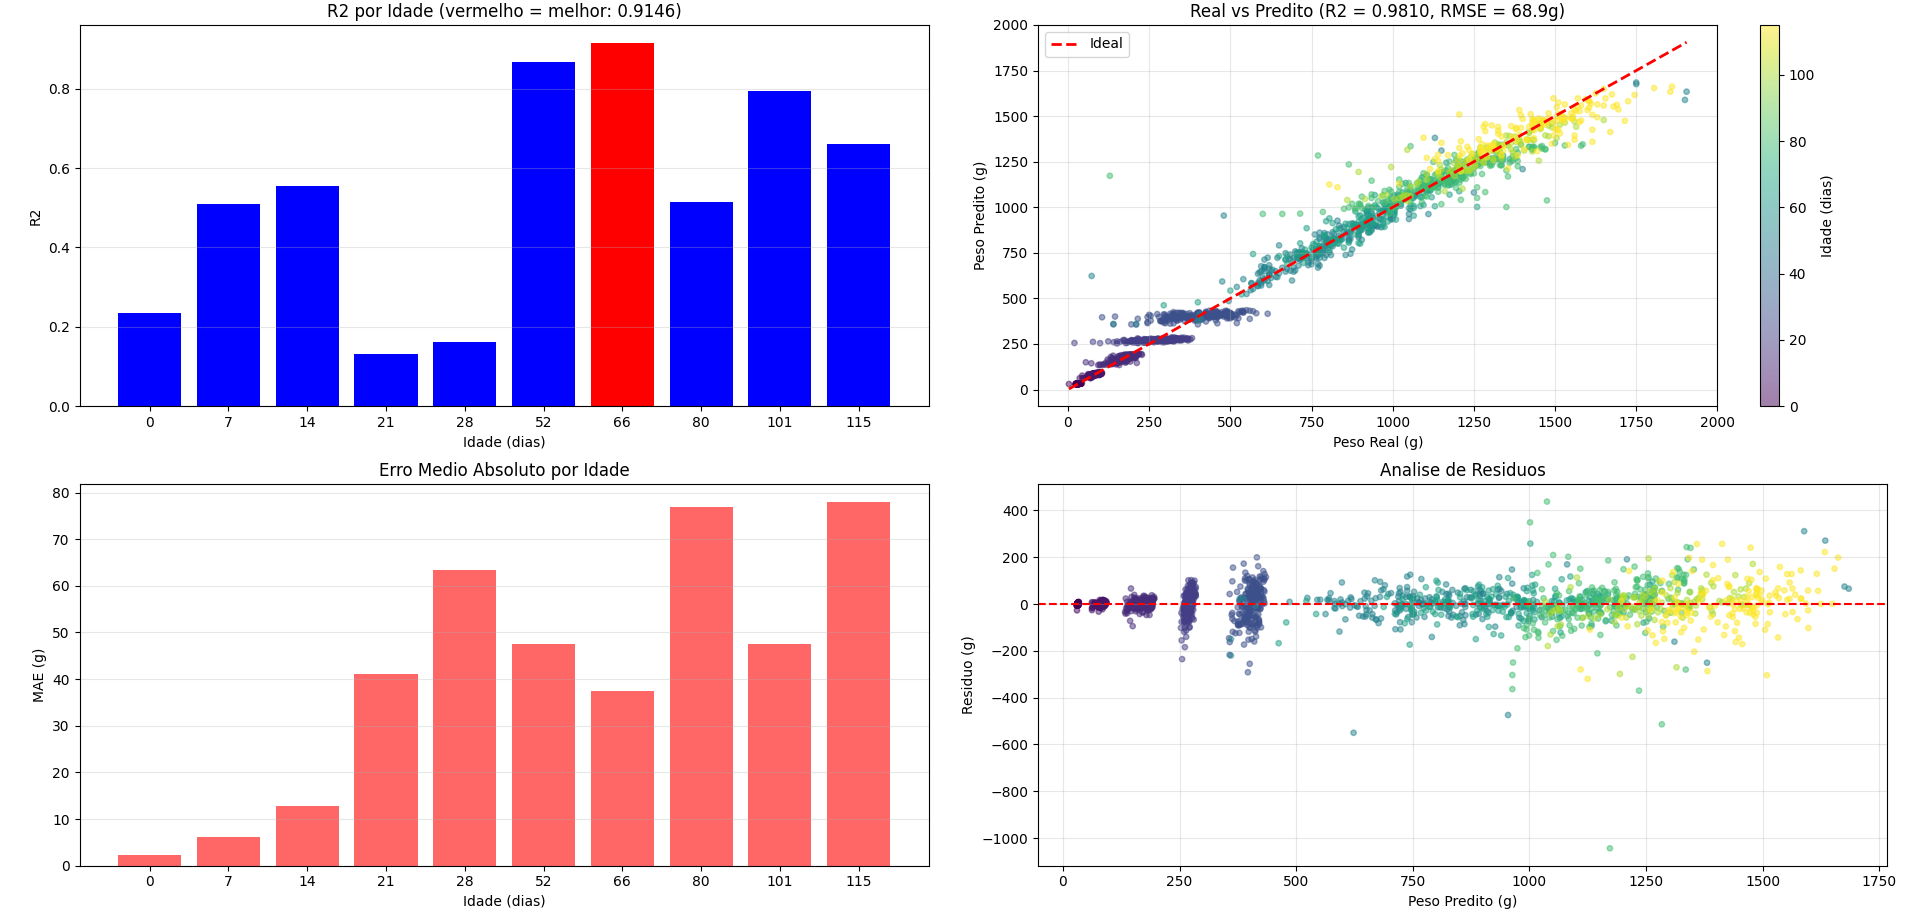
\includegraphics[width=\textwidth]{assets/fig1.png}
    \caption{Desempenho do \textit{XGBoost} na predição do peso corporal por
    faixa etária. (A) R² por idade. (B) Valores reais \textit{vs.} preditos
    (R² = 0,9810; RMSE = 68,9 g). (C) Erro absoluto médio (MAE) por idade. (D)
    Análise de resíduos.}
    \label{fig:exp1-peso}
\end{figure}

Ao analisar o desempenho por faixa etária, observou-se que o coeficiente de
determinação variou consideravelmente. A idade de 66 dias apresentou o melhor
R² individual (aproximadamente 0,91), enquanto as idades iniciais (0 e 28 dias)
apresentaram valores mais baixos (R² entre 0,13 e 0,24).

Entretanto, esse bom desempenho na idade de 66 dias deve ser interpretado com
cautela. A análise da importância das features indicou forte predominância da
variável PESO\_ANTERIOR, sugerindo que o modelo está se apoiando
majoritariamente no histórico imediato de peso, em vez de extrair padrões
relevantes a partir das medidas morfométricas. Isso limita o poder explicativo
do modelo e reduz sua capacidade de generalização em cenários onde essa
variável não esteja disponível.

O erro absoluto médio (MAE) apresentou tendência crescente com o avanço da
idade, variando de aproximadamente 2 g na idade 0 até cerca de 78 g nas idades
80 e 115 dias. Tal comportamento é esperado, uma vez que a faixa de variação do
peso corporal também aumenta com a idade. A análise de resíduos demonstrou
distribuição aproximadamente centrada em zero, porém com maior dispersão nas
idades mais avançadas.

Nas idades iniciais (0 e 7 dias), medidas como canela, circunferência abdominal
e circunferência da cabeça foram mais relevantes. A partir da idade de 14 dias,
o PESO\_ANTERIOR passou a dominar o modelo, especialmente nas idades mais
avançadas (66 a 115 dias), reforçando a dependência dessa variável.

Esses resultados são consistentes com achados da literatura, porém indicam que
o elevado R2 global (0,9810) pode estar parcialmente inflado pela presença de
variáveis altamente correlacionadas com a variável alvo, devendo ser
interpretado com cautela. Resultados semelhantes foram observados por Urooj et
al. (2023), que alcançaram R²adj = 0,999 na predição do peso de frangos Ross
308 com modelo \textit{ensemble}, e por Jahan et al. (2020), com R² = 0,9404 em
codornas japonesas utilizando redes neurais artificiais.

\subsubsection{Predição do sexo --- SVM}

O modelo SVM para classificação do sexo foi treinado e avaliado separadamente
para cada faixa etária. Os resultados revelaram desempenho altamente variável
conforme a idade das aves (Figuras~\ref{fig:exp1-sexo-f1}
e~\ref{fig:exp1-sexo-cm}).

\begin{figure}[htbp]
    \centering
    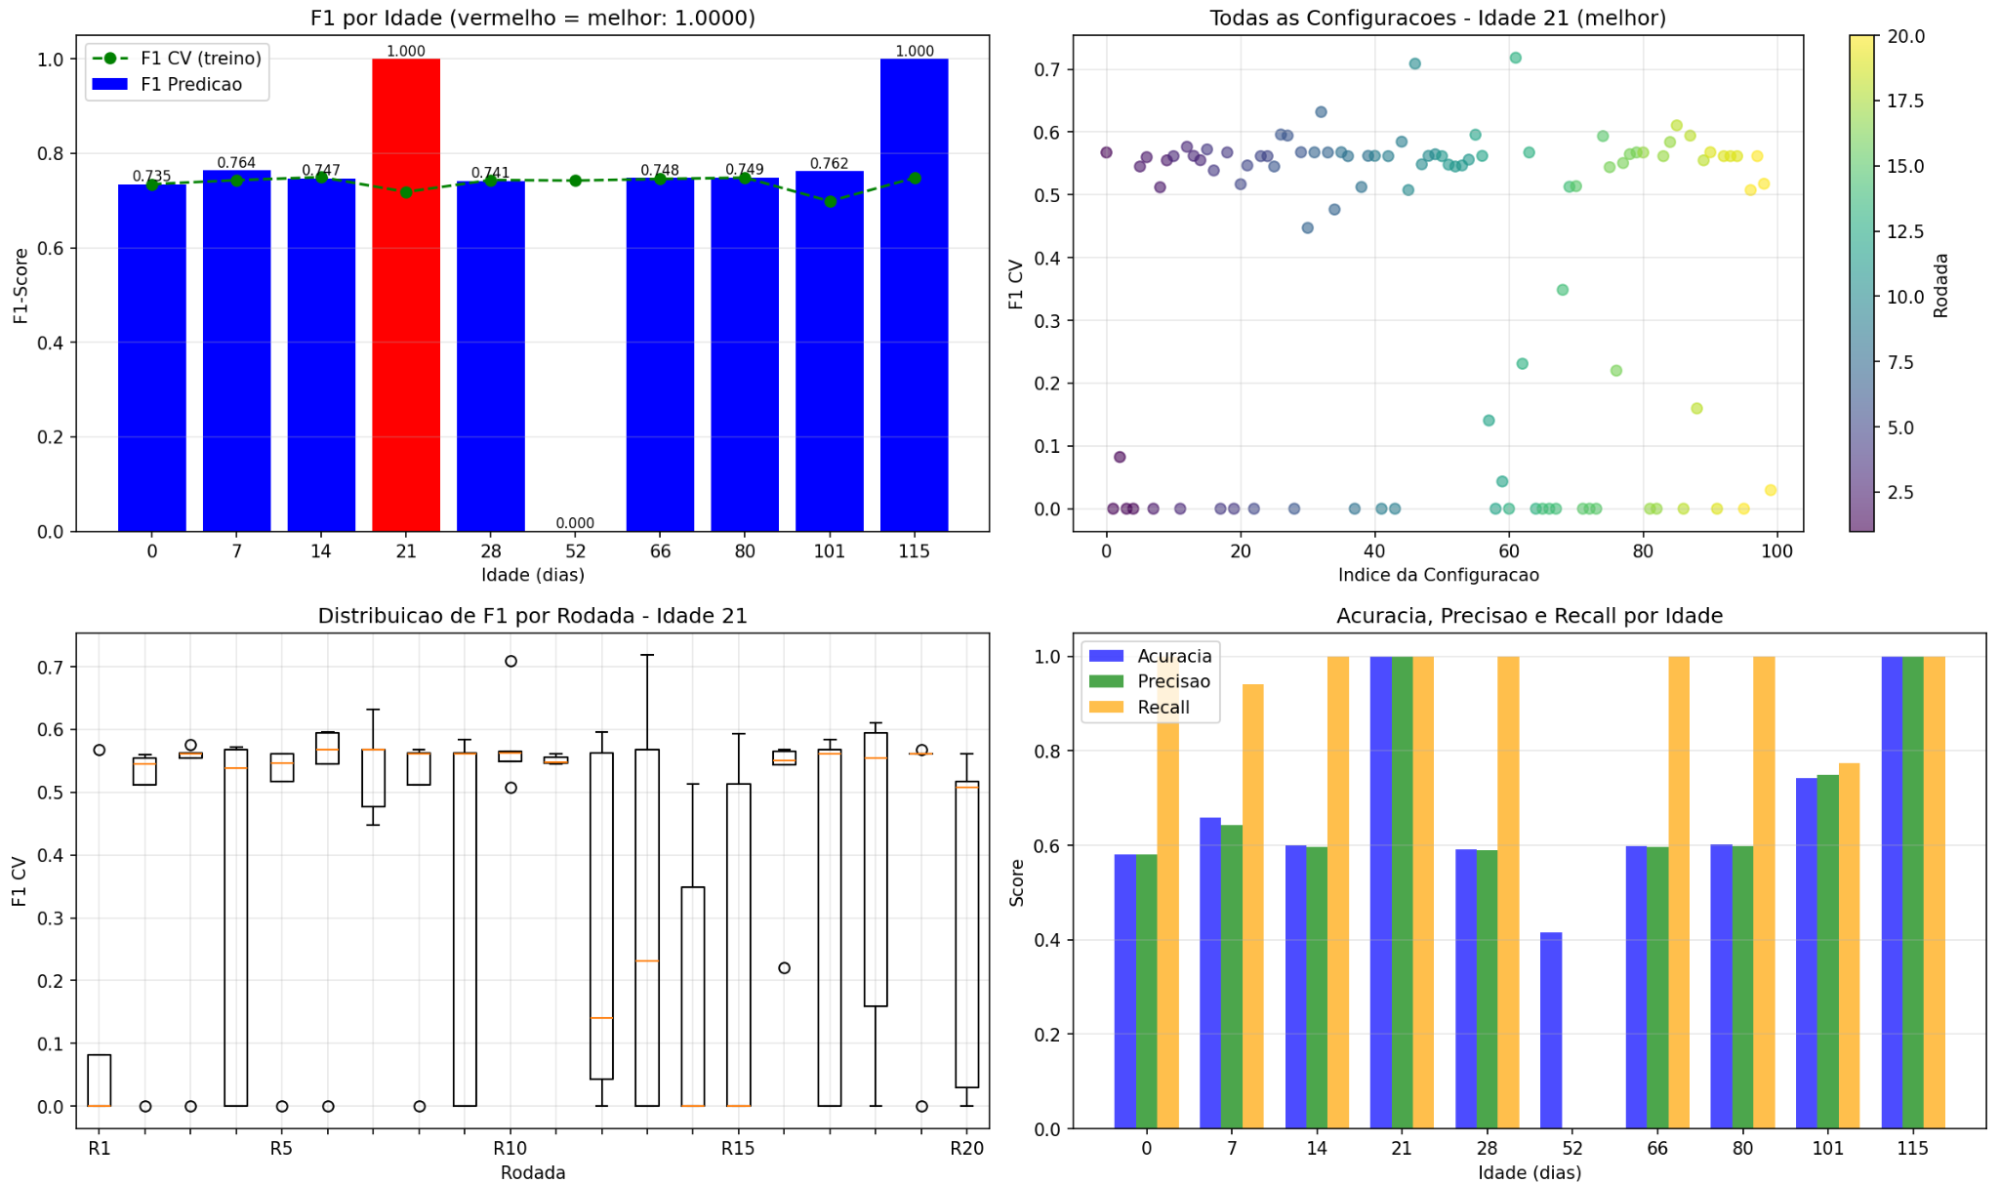
\includegraphics[width=\textwidth]{assets/fig2.png}
    \caption{Desempenho do SVM na classificação do sexo por faixa etária. (A)
    F1-Score de teste e de validação cruzada por idade. (B) F1-Score de todas
    as configurações avaliadas na melhor idade (21 dias). (C) Distribuição do
    F1-Score de validação cruzada por rodada. (D) Acurácia, precisão e
    \textit{recall} por idade.}
    \label{fig:exp1-sexo-f1}
\end{figure}

O F1-Score no conjunto de teste variou de 0,000 (idade 52) a 1,000 (idades 21 e
115). Embora as idades de 21 e 115 dias apresentem classificação perfeita,
esses resultados indicam forte evidência de sobreajuste (\textit{overfitting}),
considerando especialmente a discrepância em relação às demais idades.

Na idade de 52 dias, o modelo não obteve nenhum acerto, classificando
incorretamente todas as amostras, resultando em F1-Score nulo. Esse
comportamento sugere incapacidade do modelo em capturar padrões discriminantes
nessa faixa etária, possivelmente devido à ausência de dimorfismo sexual
significativo ou à distribuição inadequada dos dados de treino.

As matrizes de confusão evidenciam ainda um viés sistemático do modelo, com
maior capacidade de classificação de machos em comparação às fêmeas na maioria
das idades (Figura~\ref{fig:exp1-sexo-cm}).

\begin{figure}[htbp]
    \centering
    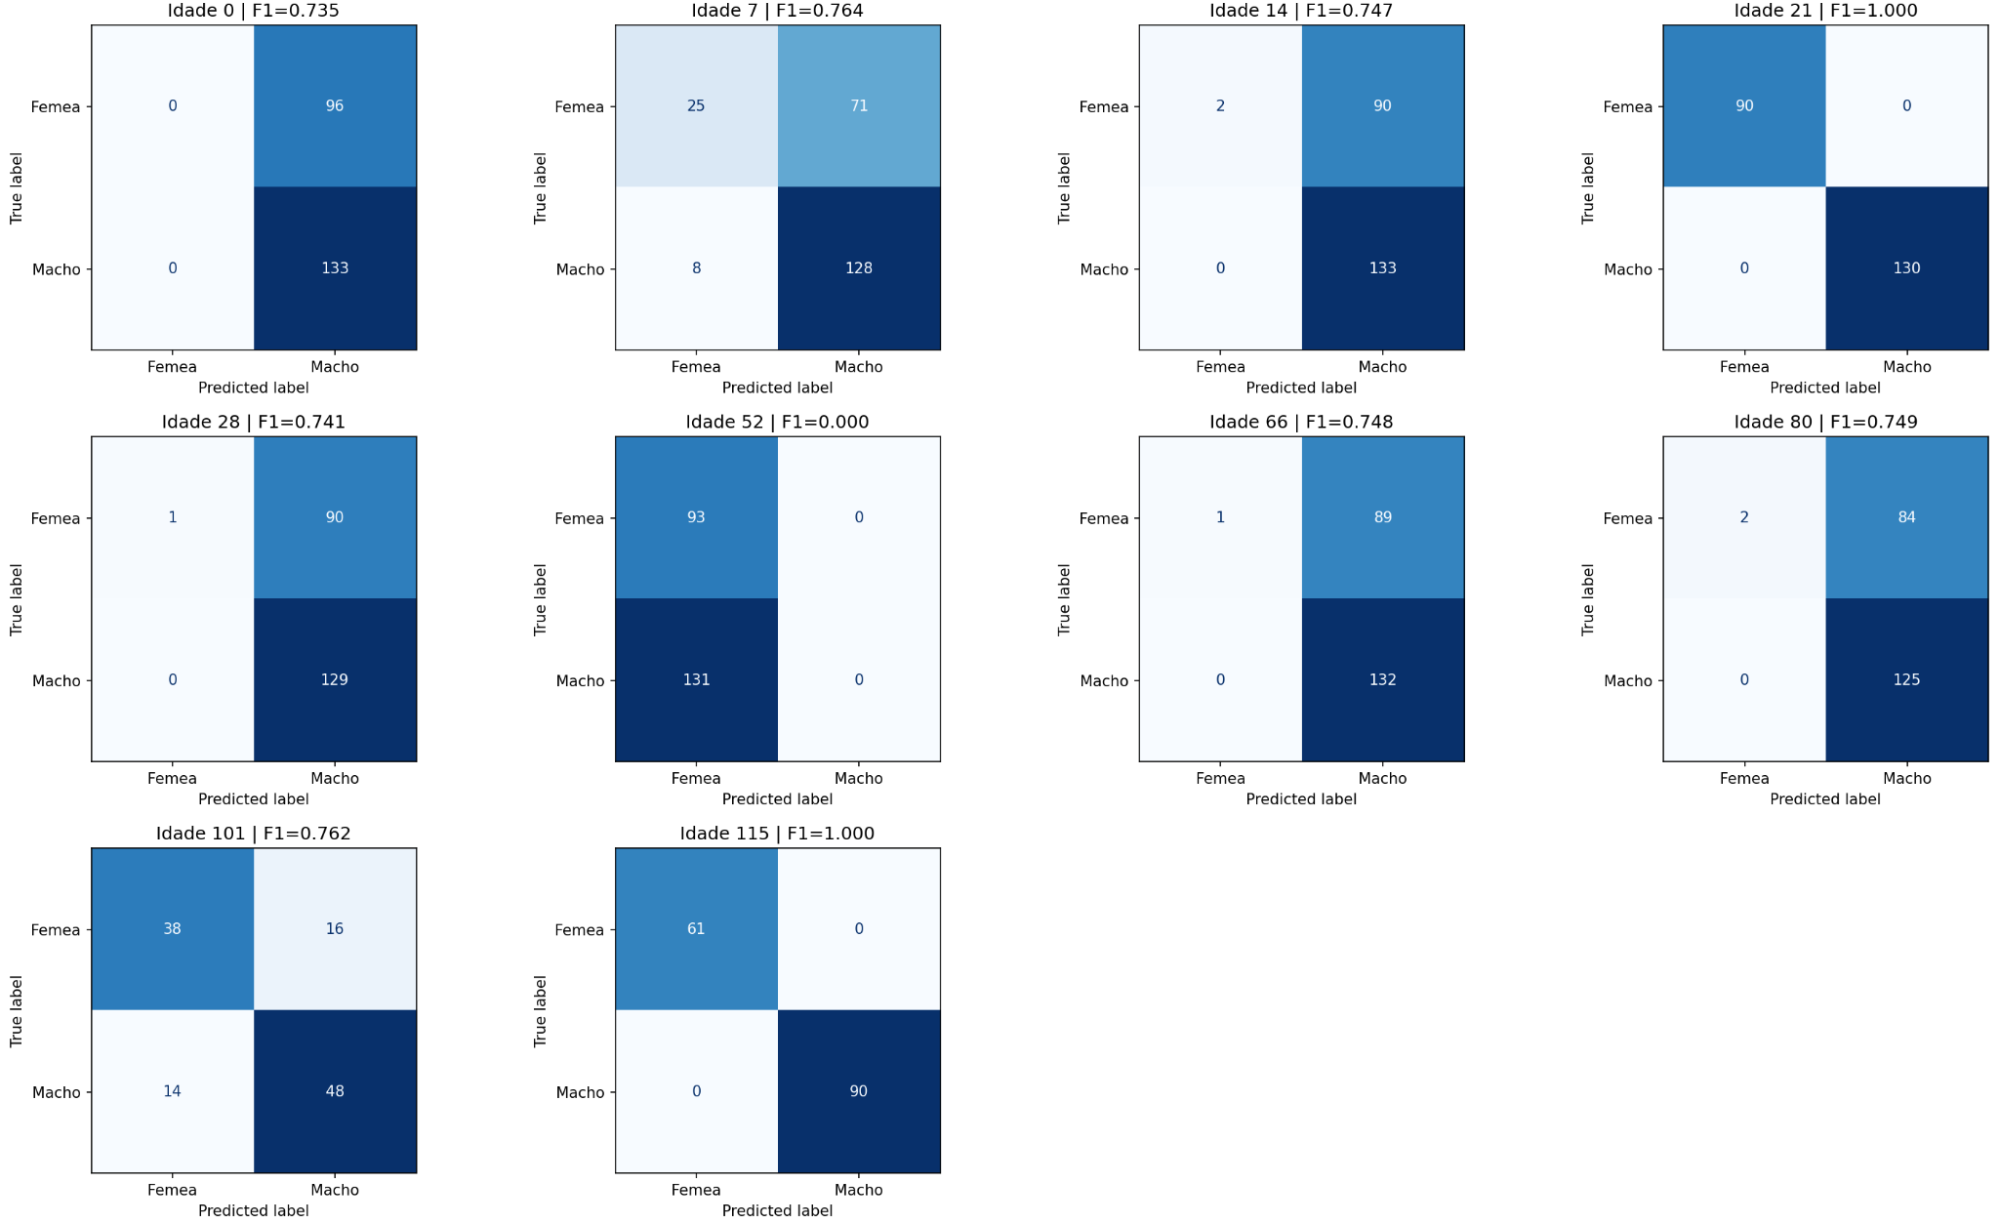
\includegraphics[width=\textwidth]{assets/fig3.png}
    \caption{Matrizes de confusão do SVM por faixa etária.}
    \label{fig:exp1-sexo-cm}
\end{figure}

Apesar de a validação cruzada no conjunto de treino apresentar F1-Score
relativamente estável (entre 0,70 e 0,76), os resultados no conjunto de teste
mostram inconsistência significativa, reforçando a presença de sobreajuste em
idades.

\subsubsection{Considerações do Experimento 1}

Os resultados do Experimento 1 indicam que o \textit{XGBoost} apresenta bom
desempenho na predição do peso corporal, porém com forte dependência da
variável PESO\_ANTERIOR, o que limita sua interpretação como modelo baseado
exclusivamente em medidas morfométricas.

Para a classificação do sexo, o SVM apresentou desempenho inconsistente, com
indícios claros de sobreajuste em algumas idades (21 e 115 dias), falha
completa em outras (52 dias) e viés na classificação em favor de machos. Esses
resultados indicam a necessidade de ajustes nos dados, balanceamento de classes
e exploração de modelos alternativos.

A dificuldade na classificação do sexo por medidas morfométricas é recorrente
na literatura. Vieira et al. (2009) destacam que ao menos metade das espécies
de aves não apresenta dimorfismo sexual evidente, e Cuan et al. (2022)
obtiveram acurácia de apenas 91,25\% na sexagem de frangos por vocalização,
demonstrando limitações dessas abordagens.

\subsection{Experimento 2}

Diferentemente do Experimento 1, neste experimento foi utilizado o conjunto de dados
completo, realizando-se uma separação manual de 20\% dos dados para teste,
garantindo o balanceamento entre machos e fêmeas. Além disso, foram avaliados
múltiplos algoritmos para a tarefa de classificação do sexo, bem como analisada
a importância das variáveis no modelo \textit{XGBoost}. Para as tarefas de
regressão e classificação finais, utilizou-se o \textit{XGBoost}.

\subsubsection{Classificação do sexo --- Comparação de modelos}

Inicialmente, foram avaliados diferentes algoritmos de classificação com o
objetivo de comparar seus desempenhos na predição do sexo das aves. Entre os
modelos testados, destacaram-se \textit{XGBoost}, \textit{LightGBM} e
\textit{KNN}, que apresentaram os melhores resultados em termos de F1-Score
(Figura~\ref{fig:exp2-sexo}).

\begin{figure}[htbp]
    \centering
    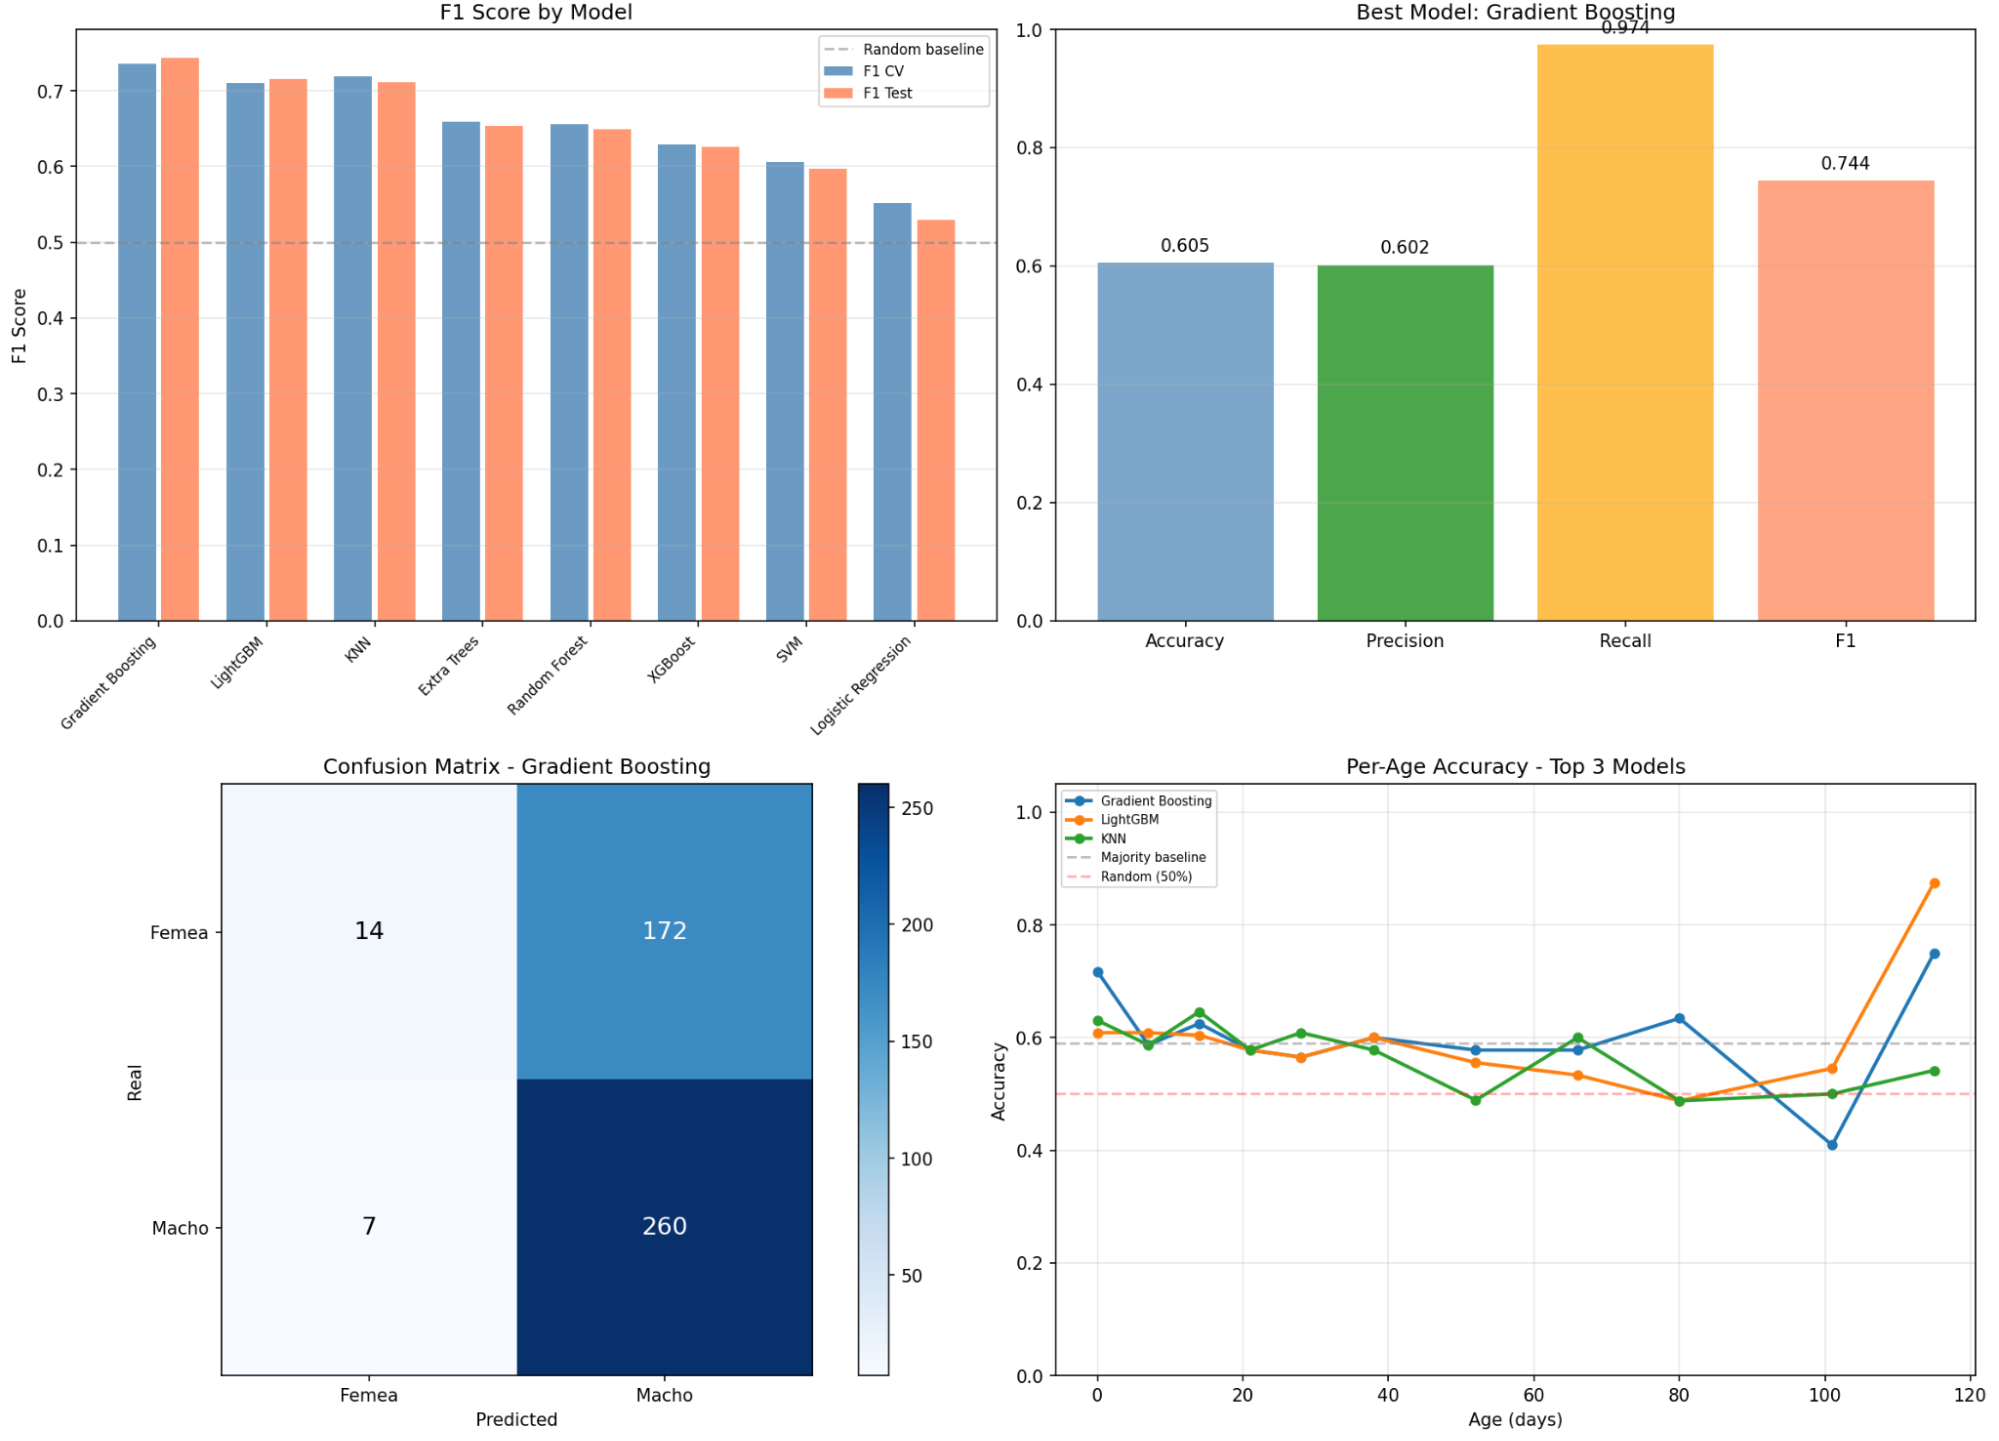
\includegraphics[width=\textwidth]{assets/fig4.png}
    \caption{Comparação entre modelos para classificação do sexo no
    Experimento 2. (A) F1-Score por modelo (CV e Teste). (B) Métricas do
    melhor modelo. (C) Matriz de confusão do melhor modelo. (D) Acurácia por
    faixa etária para os três melhores modelos.}
    \label{fig:exp2-sexo}
\end{figure}

O modelo \textit{XGBoost Classifier} apresentou o melhor desempenho geral, com
F1-Score de aproximadamente 0,744 no conjunto de teste, além de recall elevado
(0,974). No entanto, esse alto recall indica que o modelo tende a classificar
corretamente a maior parte de uma classe específica, possivelmente às custas de
erros na outra classe.

A matriz de confusão do melhor modelo evidencia um forte desbalanceamento nas
predições: a grande maioria das fêmeas foi incorretamente classificada como
machos (172 erros contra apenas 14 acertos), enquanto os machos foram
corretamente classificados em sua maioria (260 acertos).

\subsubsection{Predição do peso corporal --- XGBoost}

Para a predição do peso corporal, foi utilizado um modelo único de
\textit{XGBoost} treinado sobre todas as idades. O modelo apresentou bom
desempenho global, com R² = 0,9410 e RMSE = 113,4 g no conjunto de teste
(Figura~\ref{fig:exp2-peso}).

\begin{figure}[htbp]
    \centering
    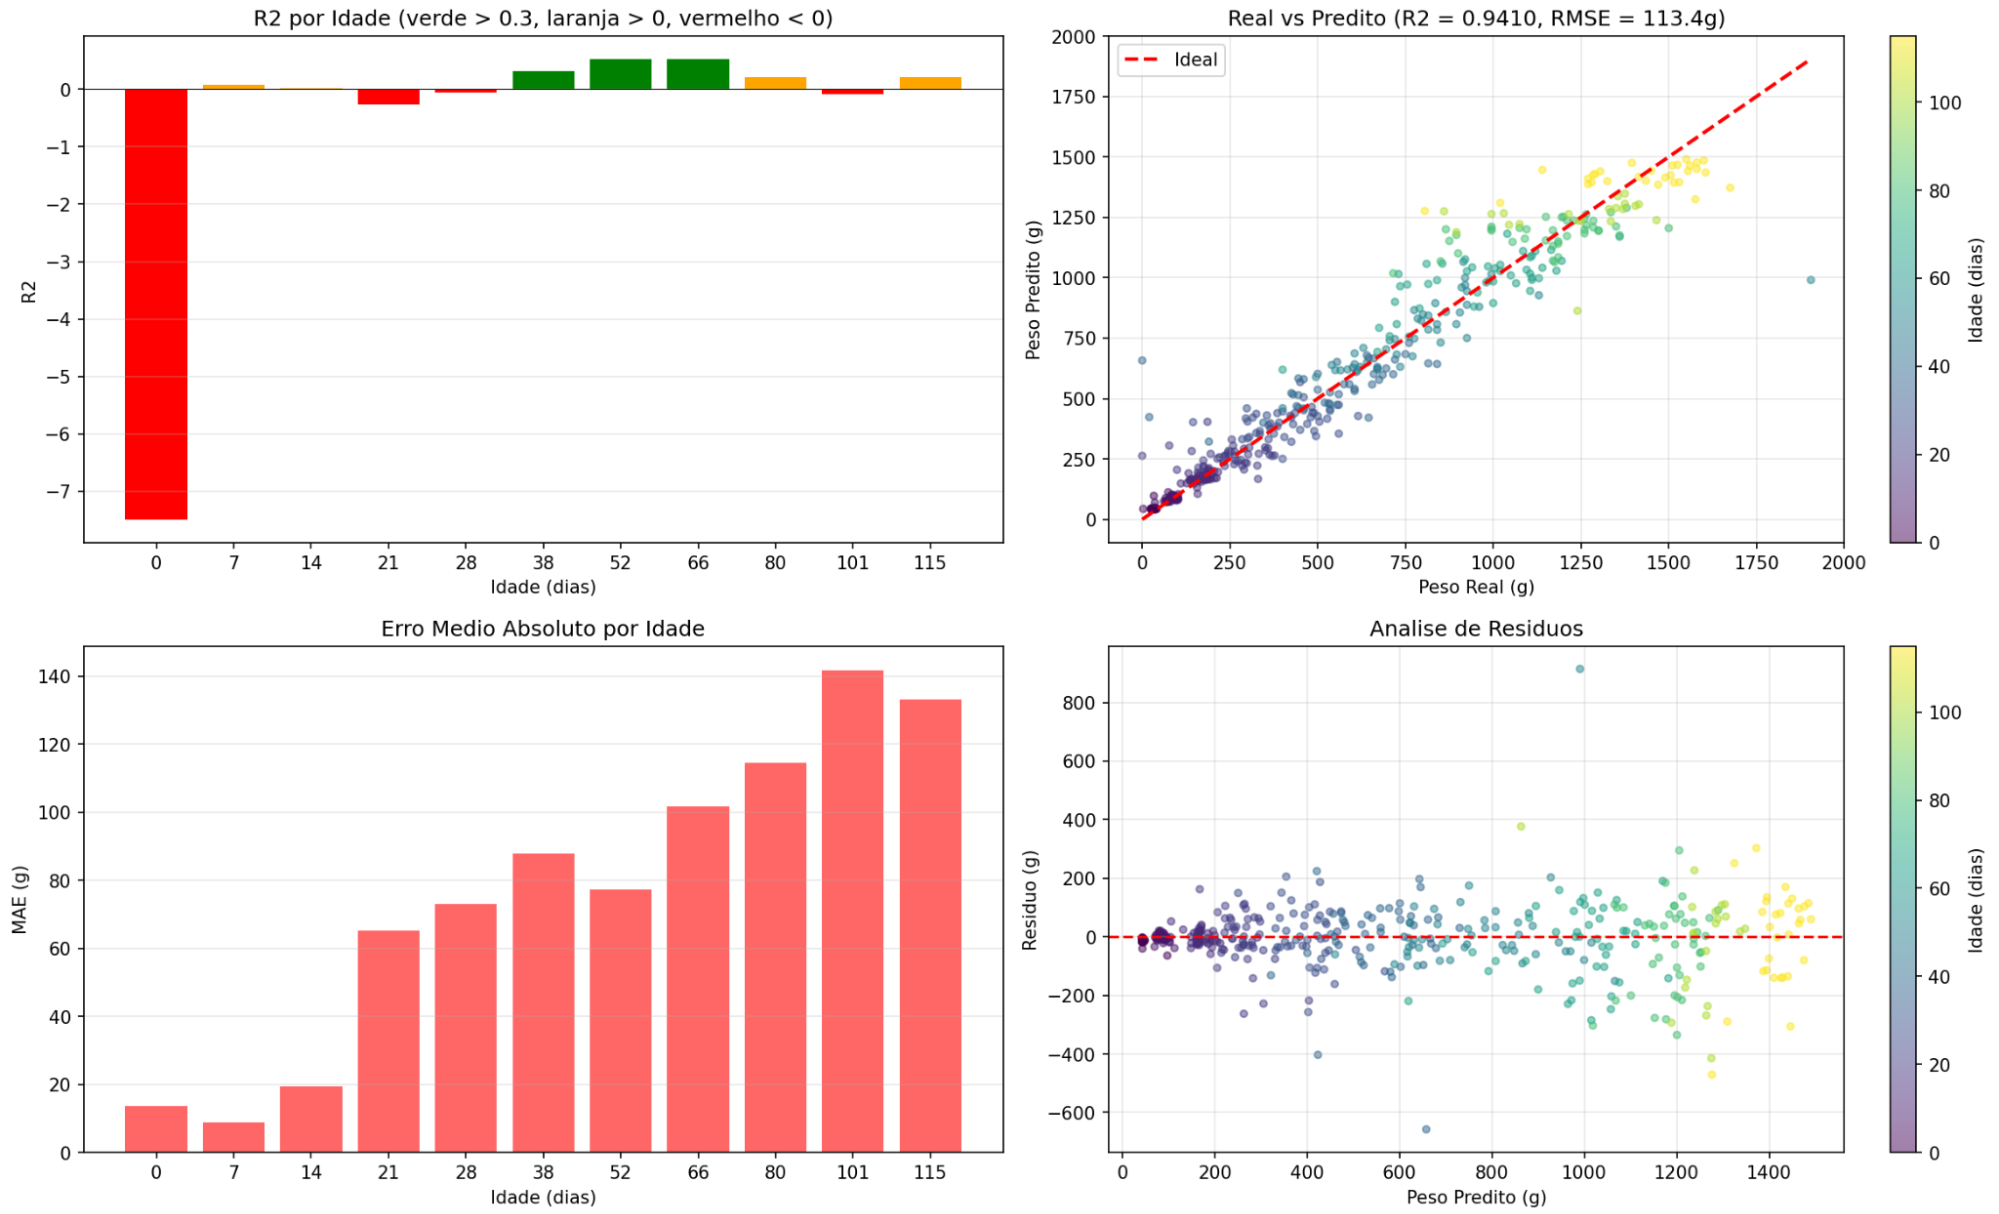
\includegraphics[width=\textwidth]{assets/fig5.png}
    \caption{Desempenho do \textit{XGBoost} na predição do peso corporal no
    Experimento 2. (A) R² por faixa etária. (B) Valores reais \textit{vs.}
    preditos (R² = 0,9410; RMSE = 113,4 g). (C) MAE por faixa etária. (D)
    Análise de resíduos.}
    \label{fig:exp2-peso}
\end{figure}

A análise por idade revelou comportamento bastante heterogêneo. A idade de 0
dias apresentou desempenho extremamente baixo (R² negativo), indicando que o
modelo não consegue capturar padrões relevantes nessa fase inicial.

O desempenho obtido é comparável ao reportado por Çakmakçi (2022), com RMSE =
4,47 em ovelhas Norduz, e por Bila (2025) em frangos Ross 308. A relevância da
circunferência abdominal como principal preditor confirma os resultados de Ogah
(2012), que identificou perímetro torácico como melhor preditor isolado (R² =
0,558) em galinhas-d'angola.

\subsubsection{Importância das variáveis --- XGBoost}

A análise da importância das features no modelo revelou que a circunferência
abdominal (CIRCFABDOM) é, de forma destacada, a variável mais relevante para a
predição do peso corporal, seguida por dorso, idade e circunferência da cabeça
(Figura~\ref{fig:exp2-importancia}).

\begin{figure}[htbp]
    \centering
    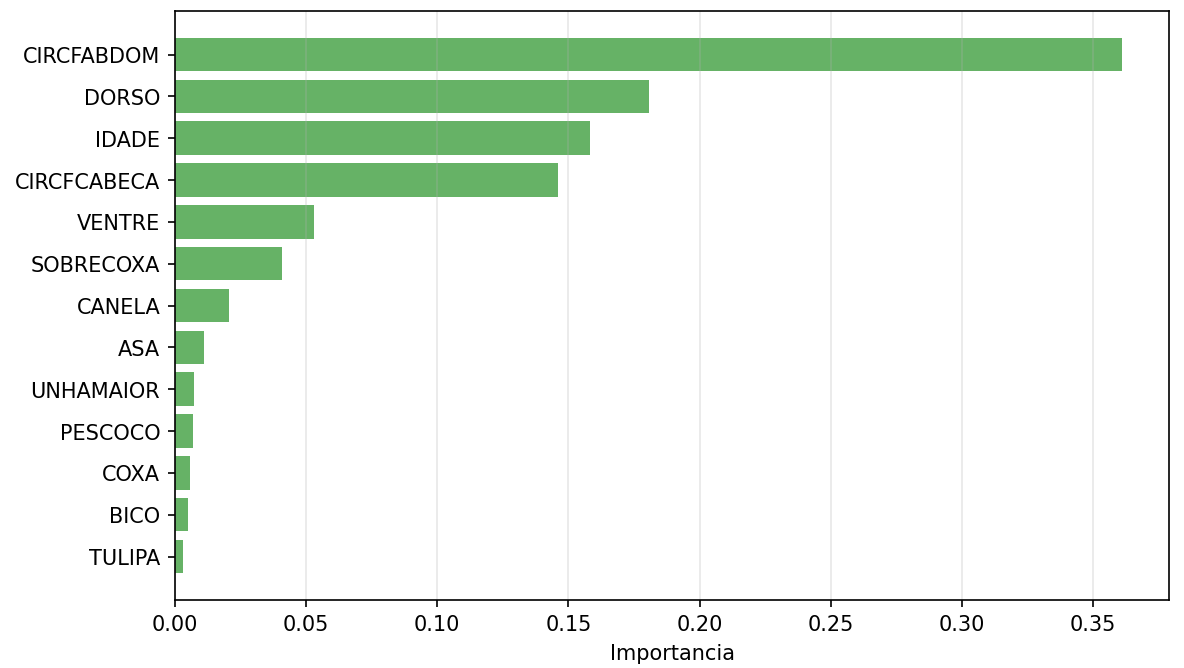
\includegraphics[width=0.9\textwidth]{assets/fig6.png}
    \caption{Importância das variáveis no modelo \textit{XGBoost} para a
    predição do peso corporal.}
    \label{fig:exp2-importancia}
\end{figure}

\subsubsection{Considerações do Experimento 2}

Os resultados do Experimento 2 indicam que, embora o uso do conjunto de dados
completo e balanceado melhore a consistência metodológica, ainda persistem
limitações importantes. Na classificação do sexo, mesmo os melhores modelos
apresentaram viés significativo, com dificuldade em identificar corretamente
fêmeas. Na predição do peso corporal, o modelo XGBoost apresentou bom
desempenho global, porém inferior ao Experimento 1. Por outro lado, essa abordagem
resulta em um modelo mais interpretável e mais robusto.

De forma geral, os resultados sugerem um compromisso entre desempenho e
capacidade de generalização.

\subsection{Experimento 3}

No Experimento 3 foi realizada uma comparação sistemática entre múltiplos
algoritmos de aprendizado de máquina para ambas as tarefas --- predição do peso
corporal e classificação do sexo ---, utilizando o conjunto de dados completo,
com separação por animal entre treino e teste. O objetivo foi identificar qual
família de algoritmos apresenta melhor desempenho no contexto biométrico das
galinhas-d'angola ao longo de todo o ciclo de crescimento, sem restrição a uma
faixa etária específica.

Em ambas as tarefas, o critério de isolamento por animal foi mantido: 20\% dos
animais foram reservados para teste (random\_state = 42), de forma que nenhuma
observação de um mesmo indivíduo ocorra simultaneamente em treino e teste. A
busca de hiperparâmetros foi conduzida por \textit{RandomizedSearchCV} em todos
os modelos.

\subsubsection{Predição do peso corporal --- Comparação de modelos}

Dez algoritmos de regressão foram avaliados: \textit{Random Forest},
\textit{Extra Trees}, \textit{Gradient Boosting}, \textit{XGBoost},
\textit{LightGBM}, \textit{KNN}, \textit{Ridge}, \textit{Lasso},
\textit{ElasticNet} e \textit{SVR}. Os preditores utilizados foram as treze
variáveis morfométricas disponíveis no conjunto de dados (bico, circunferência
da cabeça, pescoço, asa, tulipa, dorso, ventre, circunferência abdominal,
sobrecoxa, coxa, canela, unha maior e peso), acrescidas da idade (IDADE).
Diferentemente do Experimento 1, o peso registrado na mensuração anterior
(PESO\_ANTERIOR) não foi utilizado como preditor, pois o modelo opera com dados
transversais de todo o ciclo de crescimento, sem acesso ao histórico ponderal
individual.

A validação cruzada foi conduzida com \textit{KFold} (5 \textit{folds}),
adotando o R² como critério de otimização. Para mitigar o desbalanceamento
amostral entre faixas etárias, o SMOTE foi aplicado ao conjunto de treino antes
do ajuste: o alvo (PESO) foi discretizado em cinco quantis e utilizado como
rótulo auxiliar, de modo que as variáveis preditoras e o peso foram interpolados
conjuntamente na síntese de amostras.

A Tabela~\ref{tab:exp3-peso} apresenta o R² de teste de todos os modelos
avaliados. O melhor
resultado individual foi obtido pelo \textit{Random Forest}
(R²$_\text{CV}$ = 0,9447; R²$_\text{teste}$ = 0,9453; RMSE = 107,1 g;
MAE = 68,6 g), seguido de perto por \textit{Extra Trees} e
\textit{Gradient Boosting}.

\begin{table}[htbp]
\centering
\caption{Comparação de algoritmos de regressão para predição de peso corporal.}
\label{tab:exp3-peso}
\begin{tabular}{clr}
\hline
\textbf{Rank} & \textbf{Modelo} & \textbf{R² Teste} \\
\hline
 1 & Random Forest     & 0,9453 \\
 2 & Extra Trees       & 0,9449 \\
 3 & Gradient Boosting & 0,9419 \\
 4 & XGBoost           & 0,9418 \\
 5 & LightGBM          & 0,9399 \\
 6 & KNN               & 0,9393 \\
 7 & Lasso             & 0,9269 \\
 8 & Ridge             & 0,9263 \\
 9 & ElasticNet        & 0,9235 \\
10 & SVR               & 0,9162 \\
\hline
\end{tabular}
\end{table}

O desempenho global foi elevado e homogêneo entre todos os algoritmos: o
intervalo de R² variou de 0,9162 (SVR) a 0,9453 (Random Forest), diferença de
apenas 2,9 pontos percentuais. Os métodos de \textit{ensemble} baseados em
árvores (Random Forest, Extra Trees, Gradient Boosting, XGBoost e LightGBM)
concentraram-se entre as cinco primeiras posições, com R² $\geq$ 0,9399. Os
modelos lineares regularizados (Lasso, Ridge, ElasticNet) e o SVR situaram-se
nas últimas posições, porém ainda com R² > 0,91, evidenciando forte componente
linear na relação entre as medidas morfométricas e o peso.

Contudo, a análise por faixa etária para os três melhores modelos
(Figura~\ref{fig:exp3-peso}) revela comportamento marcadamente heterogêneo:
nas idades de 0 e 7 dias, o R² intra-etário colapsa para valores próximos ou
negativos, indicando que o modelo não supera um preditor trivial baseado na
média do grupo nessas fases. O R² global elevado decorre, portanto, da
dominância da variável IDADE como preditor: o modelo captura principalmente a
progressão ponderal entre faixas etárias, e não as diferenças individuais
dentro de cada faixa. Esta limitação estrutural é análoga à observada no
Experimento 2 e reforça que a estratificação por idade, adotada no
Experimento 1, é essencial para estimativas fidedignas da capacidade
preditiva real.

\begin{figure}[htbp]
    \centering
    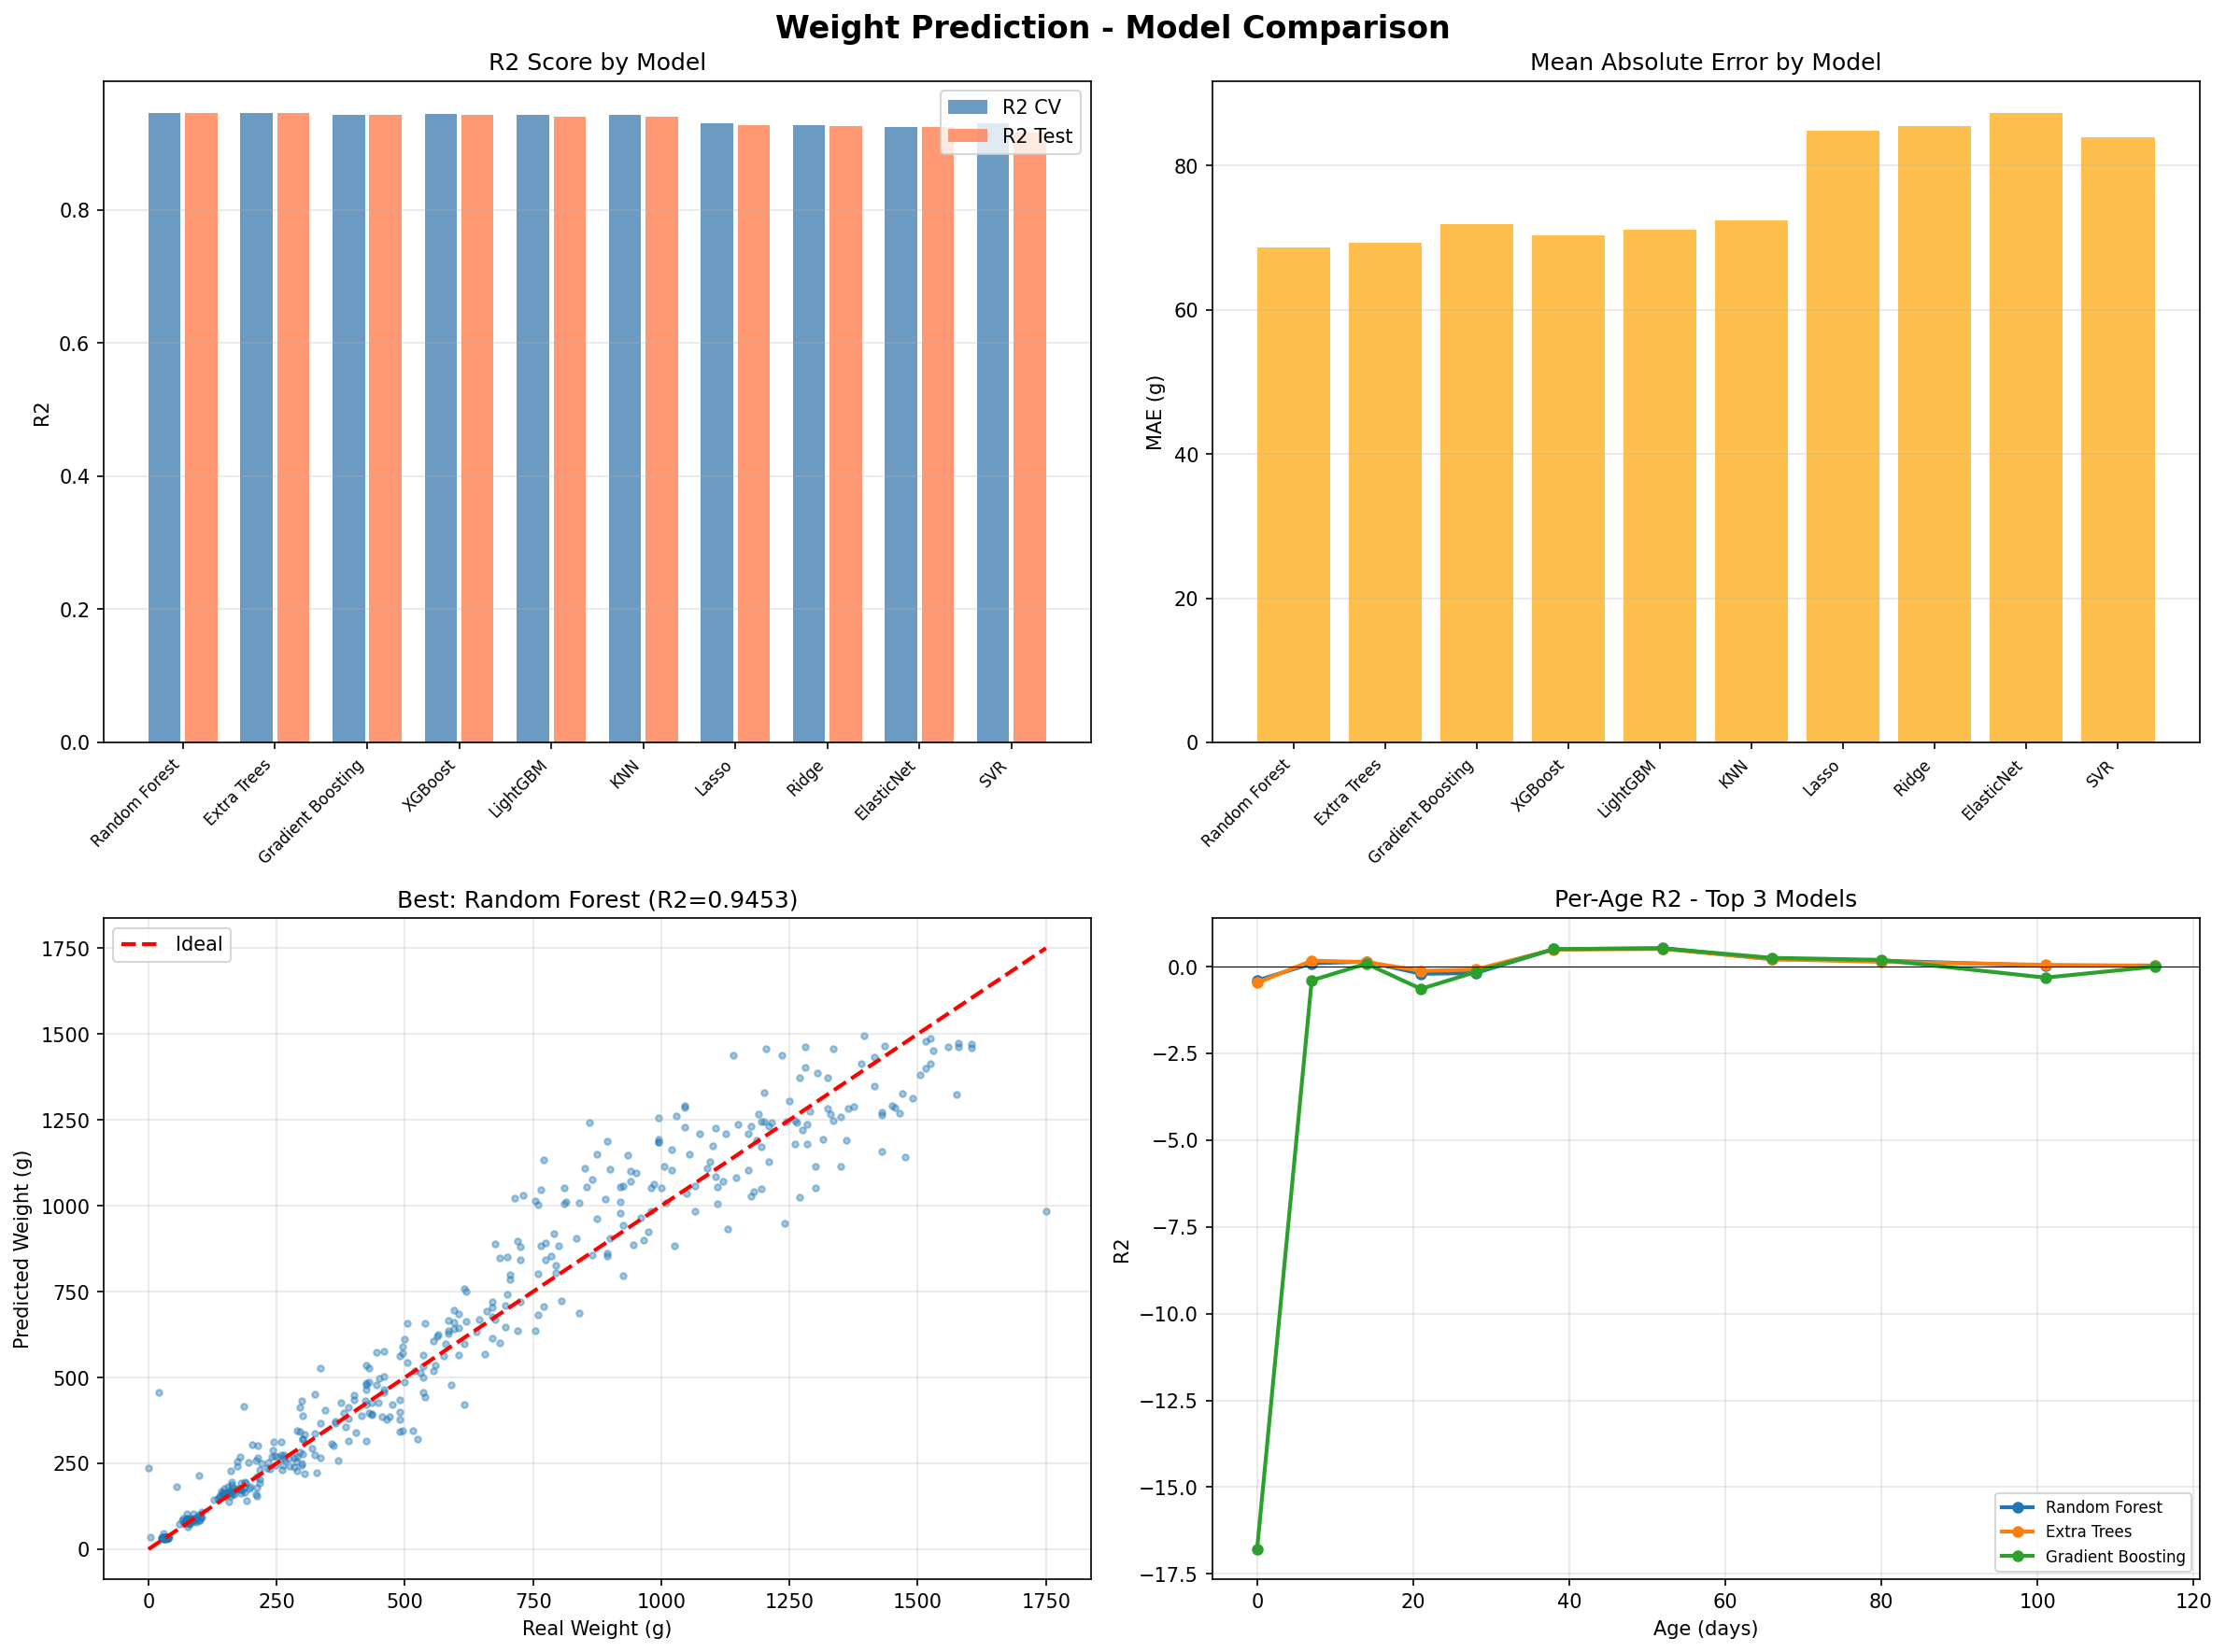
\includegraphics[width=\textwidth]{assets/fig7.png}
    \caption{Comparação de algoritmos de regressão para predição de peso
    corporal. (A) R² por modelo (CV e Teste). (B) MAE por modelo. (C) Valores
    reais \textit{vs.} preditos pelo melhor modelo (Random Forest;
    R² = 0,9453). (D) R² por faixa etária para os três melhores modelos.}
    \label{fig:exp3-peso}
\end{figure}

\subsubsection{Classificação do sexo --- Comparação de modelos}

Oito algoritmos de classificação foram avaliados: \textit{Gradient Boosting},
\textit{Random Forest}, \textit{Extra Trees}, \textit{XGBoost},
\textit{LightGBM}, SVM, \textit{KNN} e Regressão Logística. Os preditores
incluíram as treze variáveis morfométricas e a idade (IDADE), totalizando
catorze variáveis. A validação cruzada foi conduzida com
\textit{StratifiedKFold} (5 \textit{folds}), adotando o F1-Score como critério
de otimização, adequado ao desbalanceamento de classes. O SMOTE foi incorporado
diretamente ao \textit{pipeline} de cada modelo, sendo aplicado exclusivamente
dentro de cada \textit{fold} de treinamento para prevenir vazamento de dados.

A Tabela~\ref{tab:exp3-sexo} apresenta o F1-Score de teste de todos os modelos.
O melhor resultado
foi obtido pelo \textit{Gradient Boosting}, com F1$_\text{CV}$ = 0,6403, F1 de
teste = 0,6546, acurácia = 0,5784, precisão $\approx$ 0,633 e \textit{recall}
$\approx$ 0,678.

\begin{table}[htbp]
\centering
\caption{Comparação de algoritmos de classificação para predição de sexo.}
\label{tab:exp3-sexo}
\begin{tabular}{clr}
\hline
\textbf{Rank} & \textbf{Modelo} & \textbf{F1 Teste} \\
\hline
1 & Gradient Boosting   & 0,6546 \\
2 & Random Forest       & 0,6448 \\
3 & Extra Trees         & 0,6312 \\
4 & XGBoost             & 0,6250 \\
5 & LightGBM            & 0,6160 \\
6 & SVM                 & 0,5896 \\
7 & KNN                 & 0,5820 \\
8 & Regressão Logística & 0,5350 \\
\hline
\end{tabular}
\end{table}

Um resultado particularmente revelador é que a acurácia do melhor modelo
(0,5784) ficou abaixo da acurácia do classificador de maioria
(\textit{baseline} = 0,5894), indicando que nenhum algoritmo superou a
estratégia trivial de predizer sempre a classe predominante em termos de acerto
global. O F1-Score superior ao \textit{baseline} reflete que o SMOTE induziu uma
redistribuição das predições entre as classes, elevando o \textit{recall} da
classe minoritária às custas da acurácia bruta, sem que isso se traduzisse em
ganho real de discriminação.

A matriz de confusão do melhor modelo (Figura~\ref{fig:exp3-sexo}) evidencia o
padrão já observado nos experimentos anteriores: elevada taxa de erros na
classificação de fêmeas, com a maioria dos indivíduos dessa classe sendo
incorretamente classificada como macho. A análise por faixa etária revela
acentuada instabilidade: a acurácia dos três melhores modelos oscila entre 0,4
e 0,9 ao longo das dez idades, sem padrão consistente de melhora, resultado
análogo ao observado com o SVM no Experimento 1.

\begin{figure}[htbp]
    \centering
    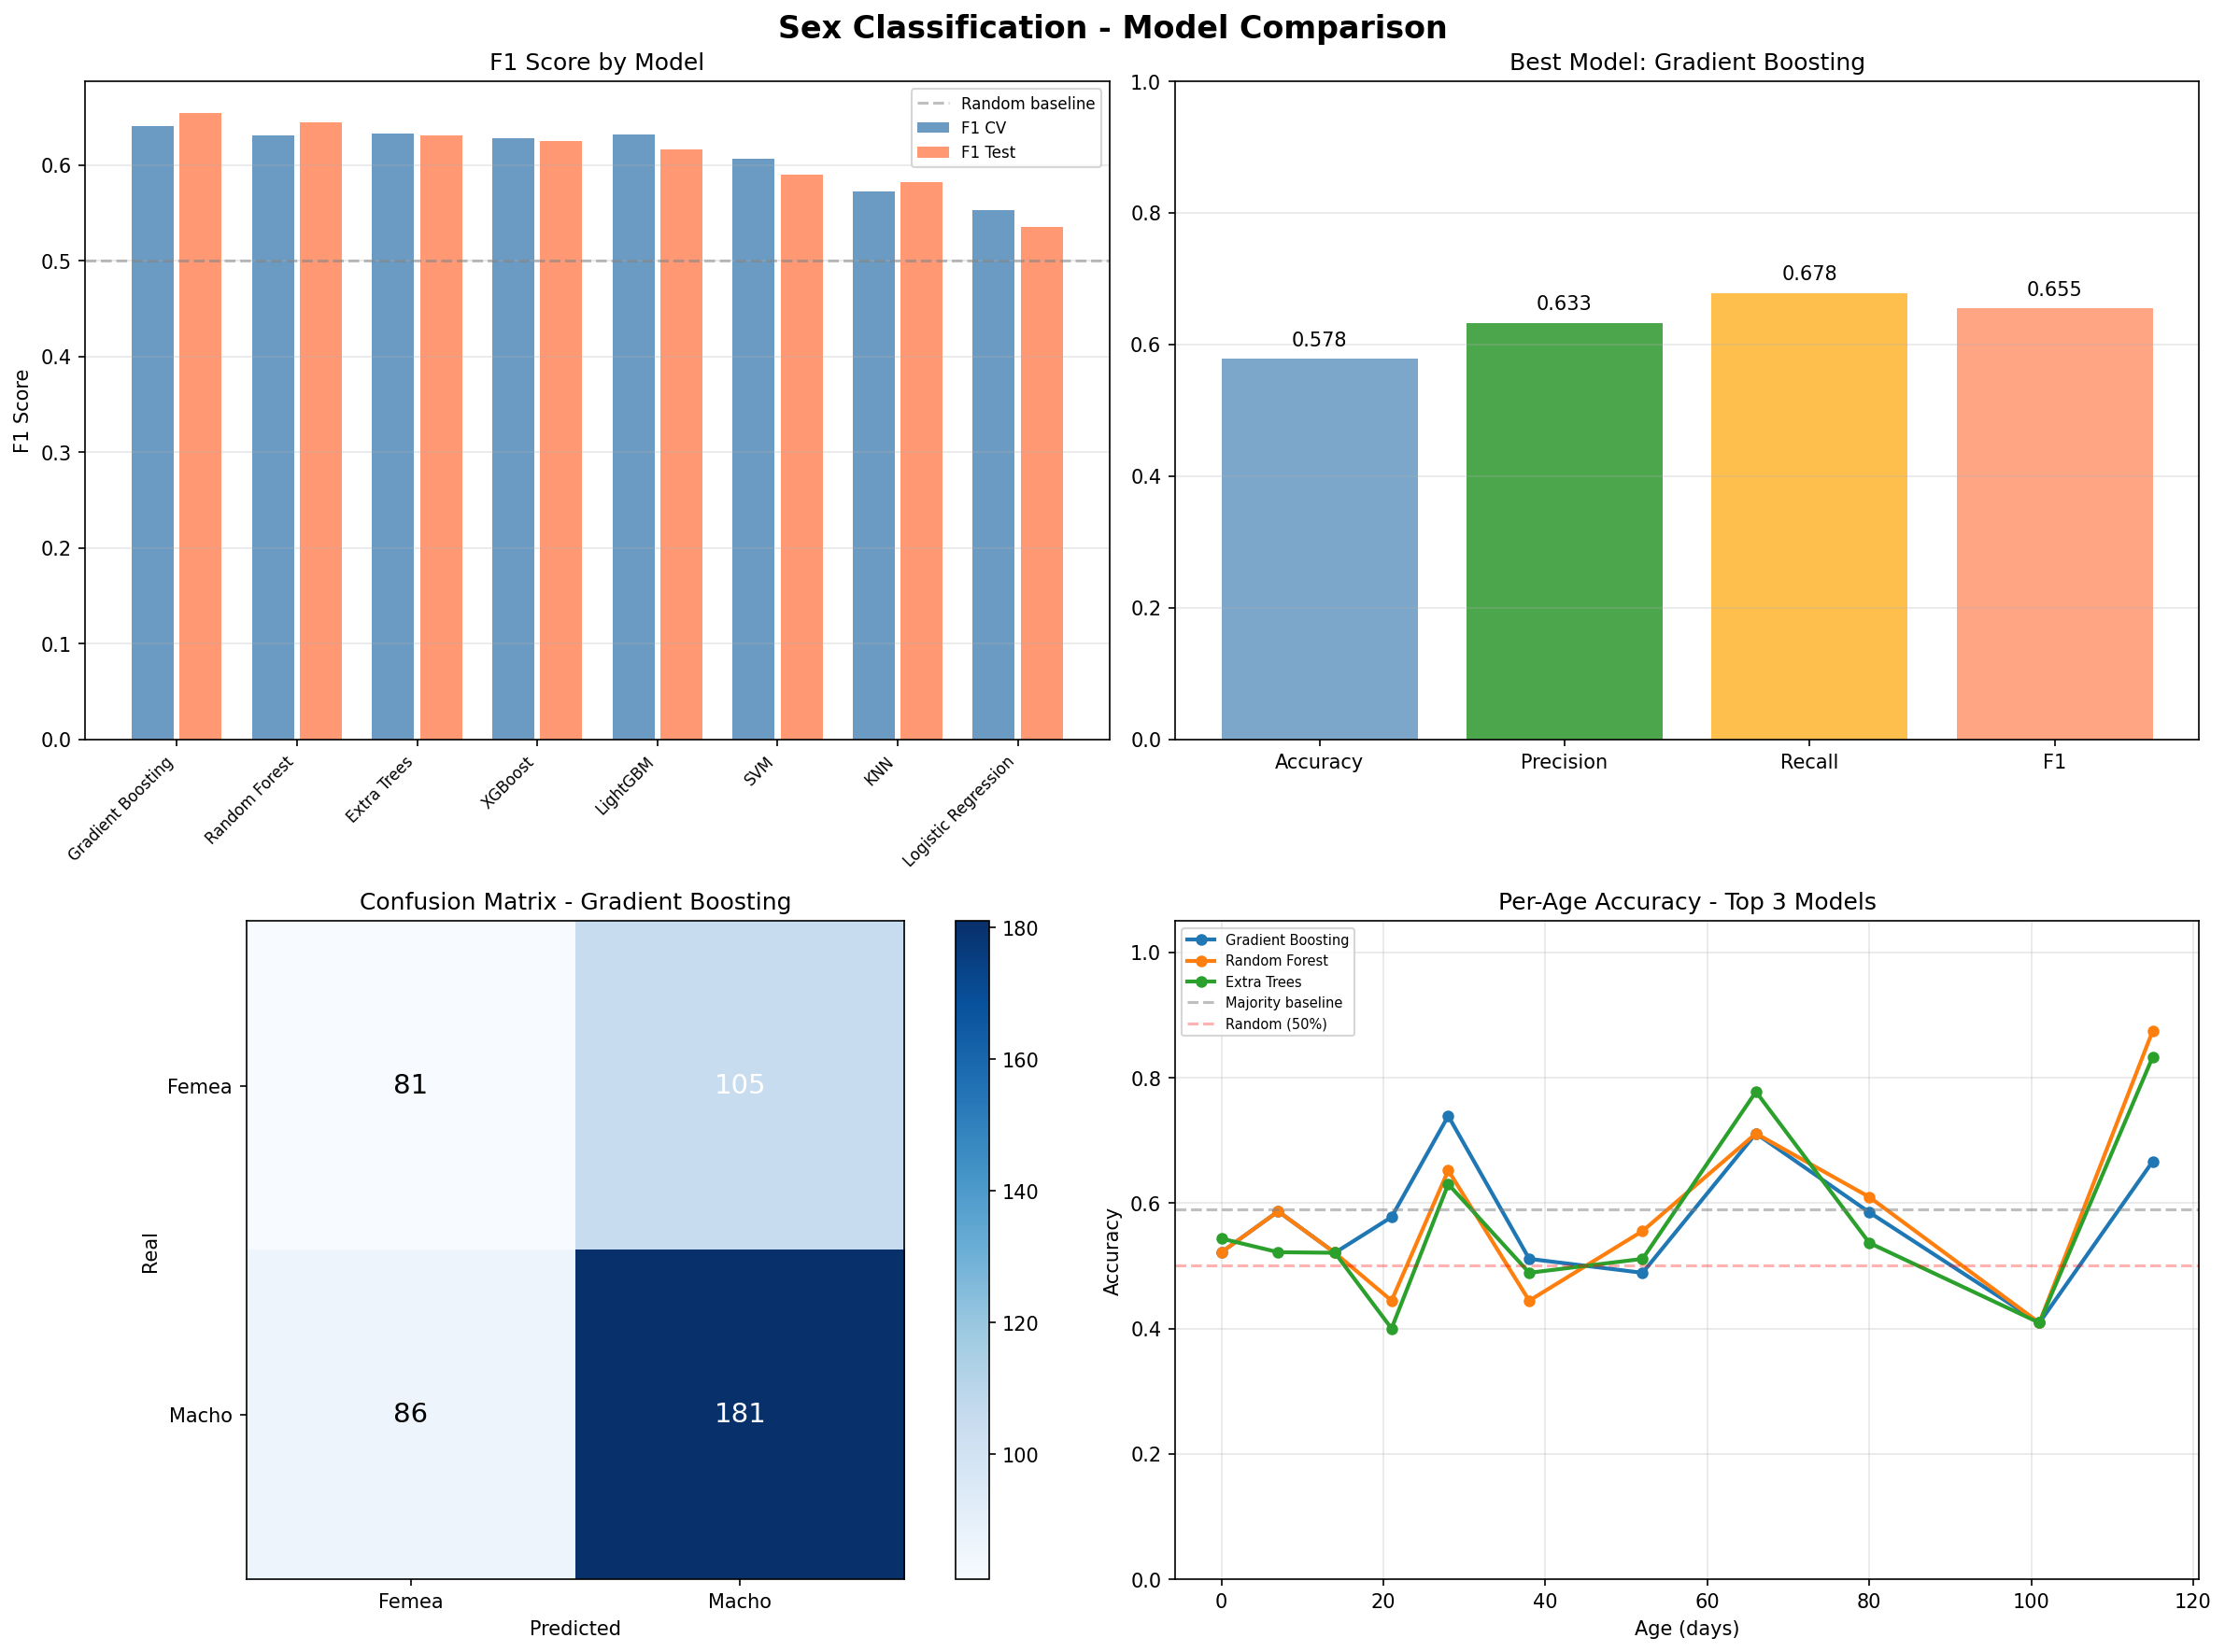
\includegraphics[width=\textwidth]{assets/fig8.png}
    \caption{Comparação de algoritmos de classificação para predição de sexo.
    (A) F1-Score por modelo (CV e Teste). (B) Métricas do melhor modelo
    (Gradient Boosting). (C) Matriz de confusão do melhor modelo. (D) Acurácia
    por faixa etária para os três melhores modelos.}
    \label{fig:exp3-sexo}
\end{figure}

\subsubsection{Considerações do Experimento 3}

O Experimento 3 corrobora e expande os achados dos experimentos anteriores. Na
predição de peso, todos os dez algoritmos avaliados atingiram R² global superior
a 0,91, com os métodos de \textit{ensemble} baseados em árvores liderando o
ranking. Todavia, o R² global é substancialmente inflado pela amplitude ponderal
entre faixas etárias, e o desempenho intra-etário é consideravelmente inferior,
em especial nos primeiros dias de vida, padrão consistente com os Experimentos 1
e 2, que reforça a superioridade da abordagem estratificada por idade para
estimativas preditivas precisas.

Na classificação do sexo, a avaliação de oito algoritmos distintos confirma que
nenhuma abordagem consegue superar o \textit{baseline} de maioria em acurácia,
independentemente do algoritmo empregado. Os resultados convergem para a
conclusão de que as medidas morfométricas disponíveis não carregam sinal
discriminatório robusto entre os sexos na maior parte do ciclo de crescimento
das galinhas-d'angola, limitação que não é contornada pela escolha do algoritmo,
pelo balanceamento via SMOTE nem pela inclusão do peso corporal como preditor.

\subsection{Experimento 4}

O Experimento 4 parte de uma ideia diferente dos anteriores. Em vez de usar as
medidas do corpo da ave, ele tenta descobrir o sexo observando como o peso da
ave evolui ao longo do tempo. A pergunta que o algoritmo busca responder é:
machos e fêmeas crescem de formas distintas o suficiente para que essa
diferença, sozinha, permita classificar o sexo?

Para responder a isso, o histórico de cada ave foi organizado em ordem de idade
e novas variáveis foram criadas para descrever o comportamento da curva de
crescimento de cada animal. Essas variáveis usam apenas dados passados da
própria ave, evitando vazamento de informação do futuro para o presente. A
Tabela~\ref{tab:exp4-features} resume cada uma delas.

\begin{table}[htbp]
\centering
\caption{Variáveis criadas a partir da relação entre idade e peso de cada ave.}
\label{tab:exp4-features}
\begin{tabular}{lp{0.62\linewidth}}
\hline
\textbf{Variável} & \textbf{O que representa} \\
\hline
IDADE & Idade da ave em dias. \\
PESO & Peso atual da ave em gramas. \\
PESO\_PRED\_MA & Média móvel dos 3 últimos pesos, usada como previsão do próximo peso. \\
PESO\_RESID & Diferença entre o peso real e o peso previsto; mostra o quanto a ave fugiu da própria tendência. \\
GANHO\_PESO & Quanto a ave engordou desde a medição anterior. \\
TAXA\_CRESC & Velocidade de crescimento, calculada como GANHO\_PESO dividido pela variação de idade. \\
TAXA\_CRESC\_MA & Média móvel da taxa de crescimento nas 3 últimas medições. \\
PESO\_ACUM\_MA & Média acumulada de todos os pesos passados da ave, que funciona como linha de base do animal. \\
SLOPE\_IA & Inclinação da reta de regressão linear entre PESO e IDADE no histórico da ave. \\
\hline
\end{tabular}
\end{table}

Depois de criar essas variáveis, o experimento testa oito algoritmos de
classificação (\textit{XGBoost}, \textit{LightGBM}, \textit{Random Forest},
\textit{Extra Trees}, \textit{Gradient Boosting}, SVM, \textit{KNN} e Regressão
Logística), todos com busca de hiperparâmetros via \textit{RandomizedSearchCV},
balanceamento por SMOTE e separação por animal, ou seja, uma mesma ave nunca
aparece ao mesmo tempo em treino e teste.

\subsubsection{Resultados}

Antes da classificação, o experimento avalia a qualidade da previsão de peso
pela média móvel. Os números mostram um erro médio absoluto de 293,74 g e um
erro quadrático médio de 329,53 g, valores altos diante da escala de pesos do
conjunto, que vai de 32 g a quase 1500 g. Isso já indica que a curva de
crescimento é bastante variável dentro do mesmo animal. A comparação dos modelos
é apresentada na Tabela~\ref{tab:exp4-modelos}.

\begin{table}[htbp]
\centering
\caption{Comparação dos modelos de classificação no Experimento 4, ordenados por
F1 no teste.}
\label{tab:exp4-modelos}
\begin{tabular}{lccc}
\hline
\textbf{Modelo} & \textbf{F1 Validação} & \textbf{F1 Teste} & \textbf{Acurácia} \\
\hline
\textbf{Extra Trees} & \textbf{0,633} & \textbf{0,564} & \textbf{0,558} \\
XGBoost & 0,594 & 0,544 & 0,549 \\
Random Forest & 0,610 & 0,532 & 0,547 \\
Gradient Boosting & 0,613 & 0,527 & 0,549 \\
LightGBM & 0,616 & 0,510 & 0,531 \\
SVM & 0,533 & 0,489 & 0,503 \\
KNN & 0,489 & 0,487 & 0,509 \\
Regressão Logística & 0,494 & 0,427 & 0,475 \\
\hline
\end{tabular}
\end{table}

O melhor modelo foi o \textit{Extra Trees}, com F1 de 0,564 no teste e acurácia
de 0,558. A linha de base, que consiste em sempre prever a classe majoritária,
atinge 0,442 de acurácia, então o modelo fica cerca de 11 pontos percentuais
acima desse piso.

Observando a matriz de confusão do \textit{Extra Trees}, o modelo acertou 103
fêmeas e 108 machos, mas confundiu 108 fêmeas como machos. A revocação
(\textit{recall}) alta (0,647) com precisão baixa (0,500) mostra que ele tende a
inclinar suas predições para a classe positiva, errando bastante quando o faz.

O gráfico das curvas de crescimento médio por sexo, apresentado no painel
inferior direito da Figura~\ref{fig:exp4-sexo}, deixa claro o motivo dessa
dificuldade. As duas curvas, de machos e fêmeas, estão praticamente
sobrepostas em todas as idades. Em outras palavras, na média, a velocidade e o
formato do crescimento são quase idênticos entre os sexos, de modo que as
variáveis derivadas dessa curva não conseguem separar bem as classes.

\begin{figure}[htbp]
    \centering
    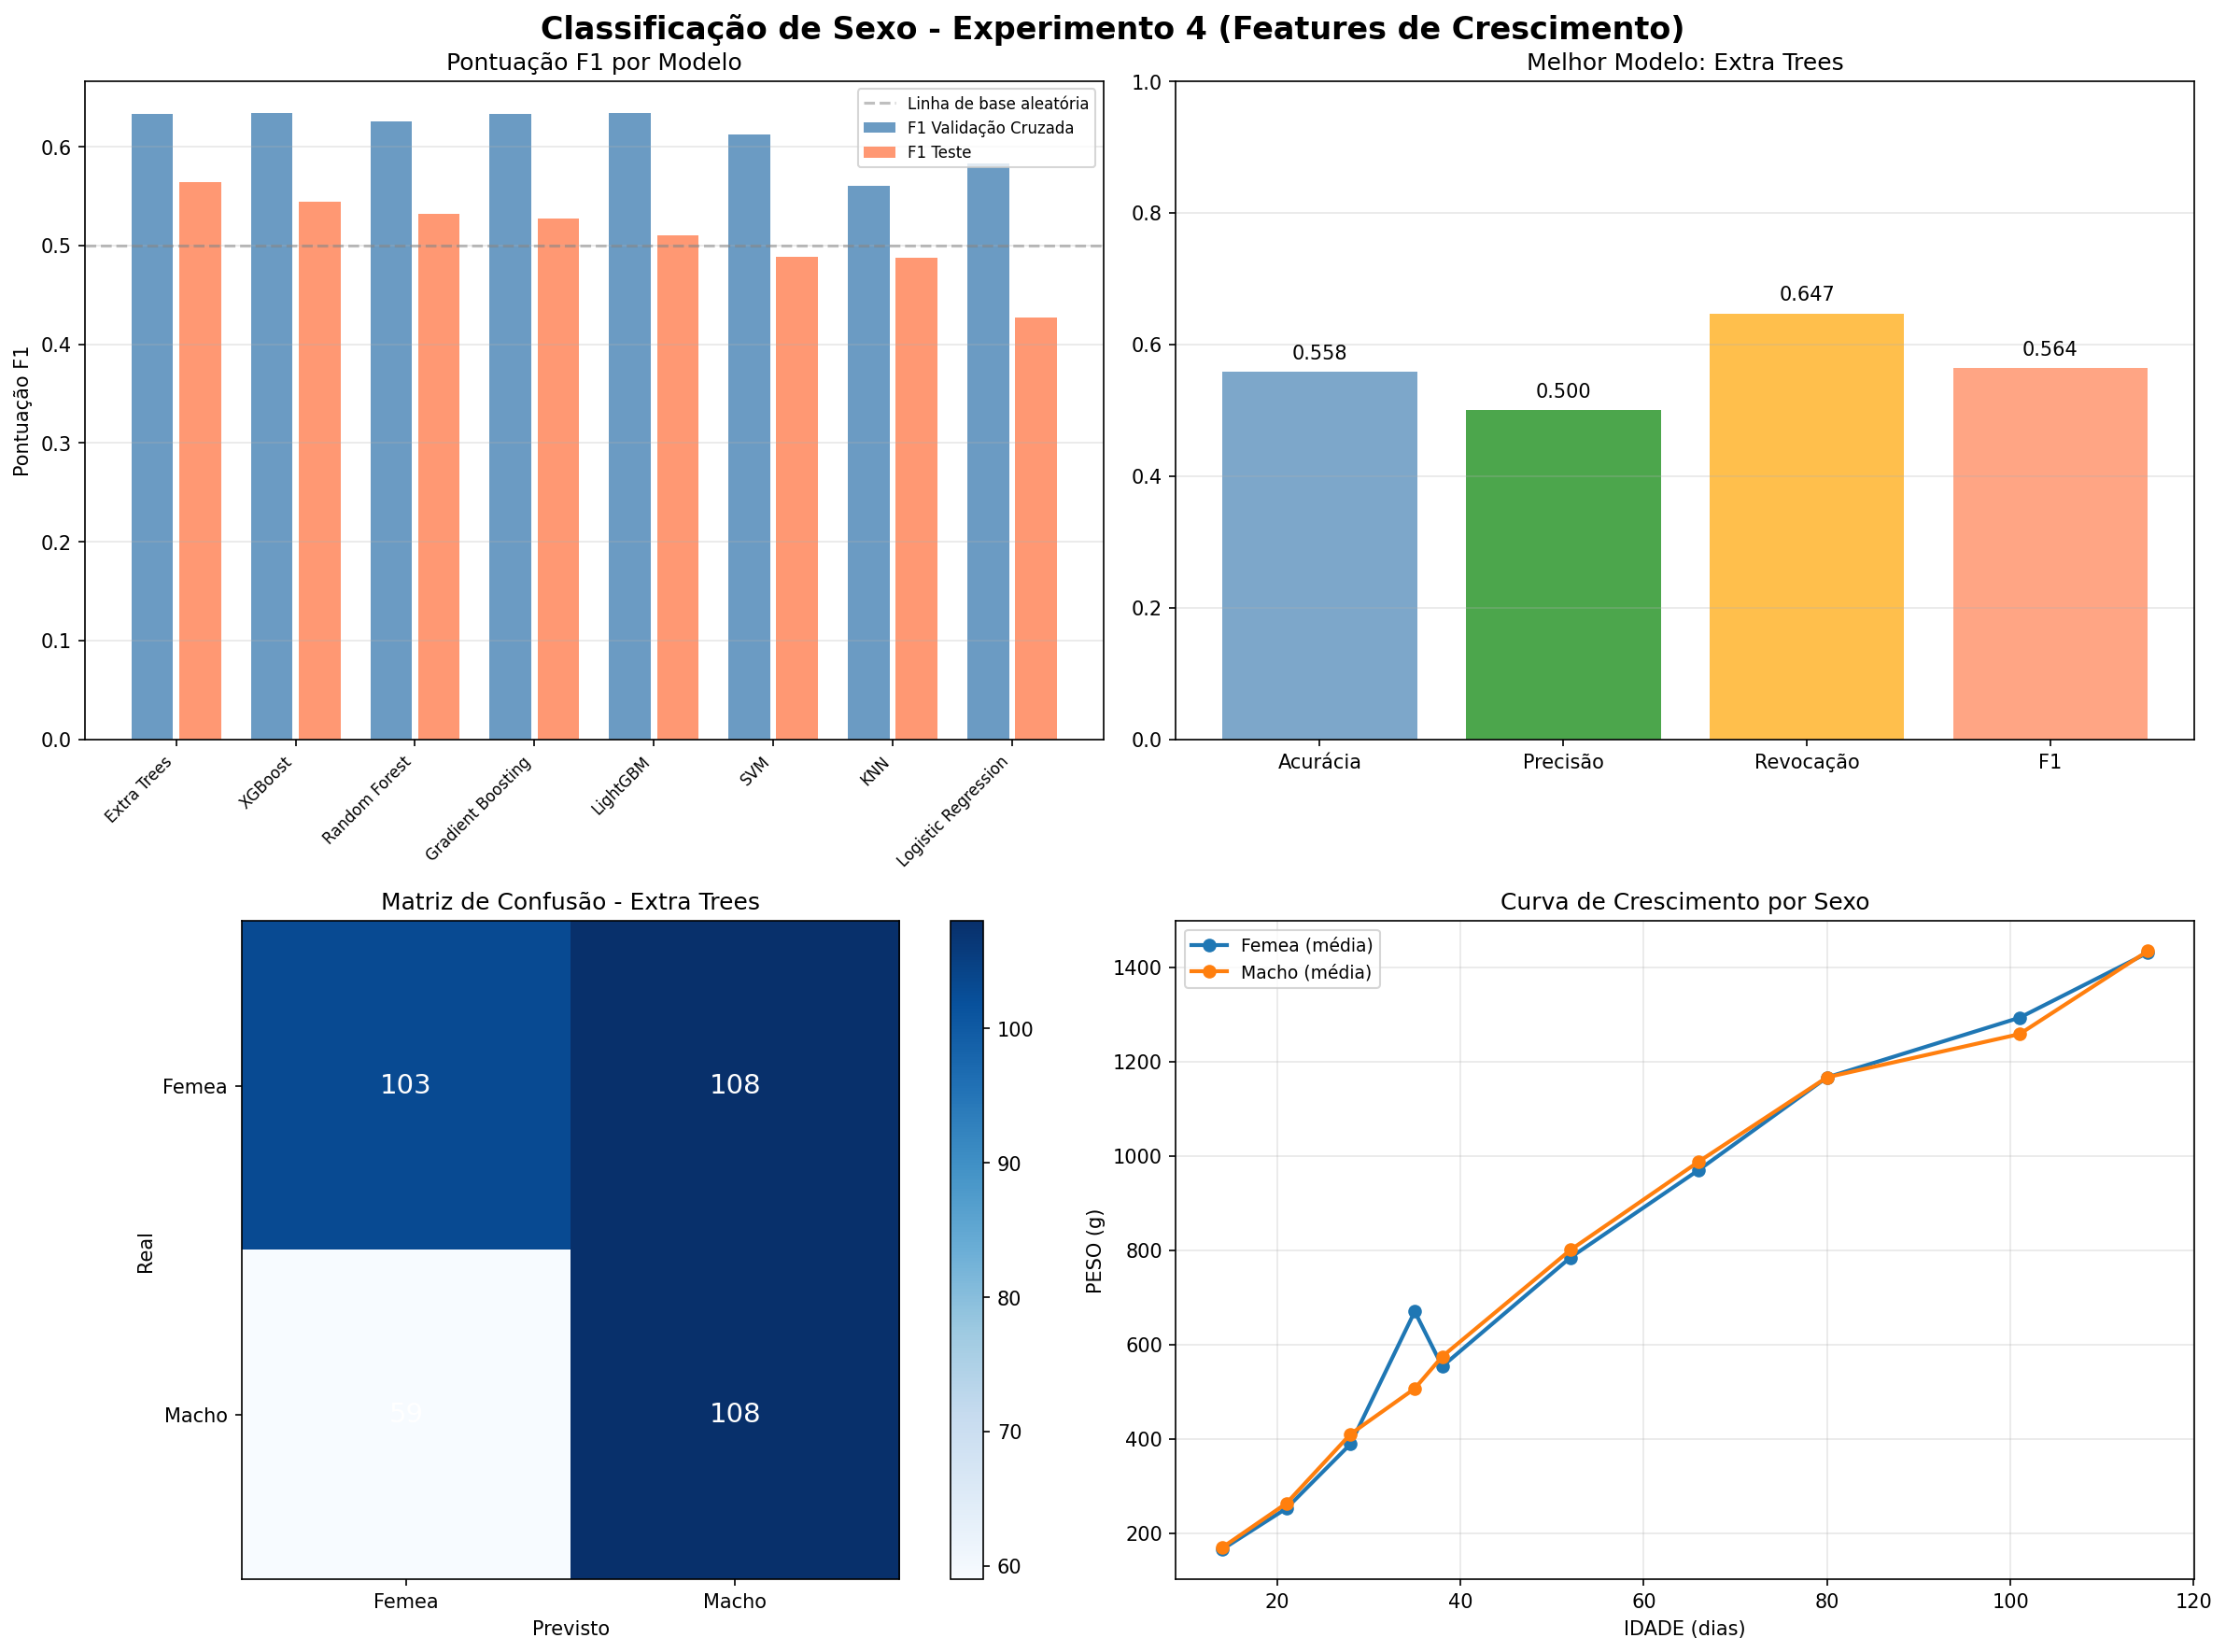
\includegraphics[width=\textwidth]{assets/fig9.png}
    \caption{Resultados do Experimento 4: comparação dos modelos, métricas do
    melhor modelo, matriz de confusão e curvas de crescimento por sexo.}
    \label{fig:exp4-sexo}
\end{figure}

\subsubsection{Considerações do Experimento 4}

O experimento mostra que, mesmo trocando o tipo de informação usada ---
abandonando as medidas do corpo e olhando apenas para a relação entre idade e
peso ---, ainda não é possível classificar o sexo das aves com qualidade. O
modelo ganha algum sinal sobre a \textit{baseline}, mas fica longe de um
resultado prático, e só funciona um pouco porque captura pequenas diferenças
individuais, não porque exista um padrão consistente de crescimento por sexo.

Esse resultado reforça a conclusão central da pesquisa: a galinha-d'angola é uma
espécie monomórfica, ou seja, machos e fêmeas se desenvolvem com tamanhos e
curvas de crescimento muito parecidos, e por isso variáveis morfométricas,
sozinhas ou combinadas em \textit{features} de crescimento, não bastam para
distinguir o sexo de forma confiável.

\subsection{Experimento 5}

Os testes anteriores indicaram que o alto valor de R² geral na estimativa do peso corporal poderia estar inflado por variáveis muito ligadas ao alvo, que são PESO\_ANTERIOR no Experimento 1 e IDADE nos Experimentos 2 e 3. O Experimento 5 testa essa hipótese e, ao mesmo tempo, verifica quantas medidas corporais são realmente necessárias. Duas mudanças principais diferenciam este experimento dos outros: a variável IDADE foi retirada dos preditores e o desempenho passou a ser medido também dentro de cada faixa etária. A base contou com 2.279 registros em onze idades, divididos por animal (190 aves para treino e 48 para teste), usando o ajuste de hiperparâmetros do \textit{XGBoost} por \textit{RandomizedSearchCV} com \textit{KFold} de cinco partes.

\subsubsection{Seleção das variáveis mais importantes}

Um primeiro modelo, treinado com as doze medidas corporais, organizou as variáveis pela importância de ganho (\textit{gain}). Escolheu-se o menor grupo de variáveis cuja importância somada chegasse a 95\%, o que resultou em sete medidas: CIRCFABDOM (0,538), CIRCFCABECA (0,209), SOBRECOXA (0,063), DORSO (0,059), ASA (0,037), UNHAMAIOR (0,029) e VENTRE (0,025). As cinco medidas deixadas de fora, que foram PESCOCO, COXA, BICO, CANELA e TULIPA, somam apenas 4,1\% do peso total. Chama a atenção essa concentração: a circunferência do abdômen e a circunferência da cabeça juntas respondem por 74,7\% do resultado, o que concorda com o Experimento 2 e com o trabalho de Ogah (2012), que apontou o perímetro do peito como a melhor medida individual para estimar o peso em galinhas-d'angola.

Treinado de novo apenas com essas sete variáveis, o modelo manteve o mesmo desempenho do conjunto completo (R²$_\text{teste}$ = 0,9388 contra 0,9391 com as doze medidas; RMSE de 113,3 g contra 113,0 g), como mostra a Figura~\ref{fig:exp5-features}. A redução no número de variáveis, portanto, não causou perda de precisão.

\begin{figure}[htbp]
\centering
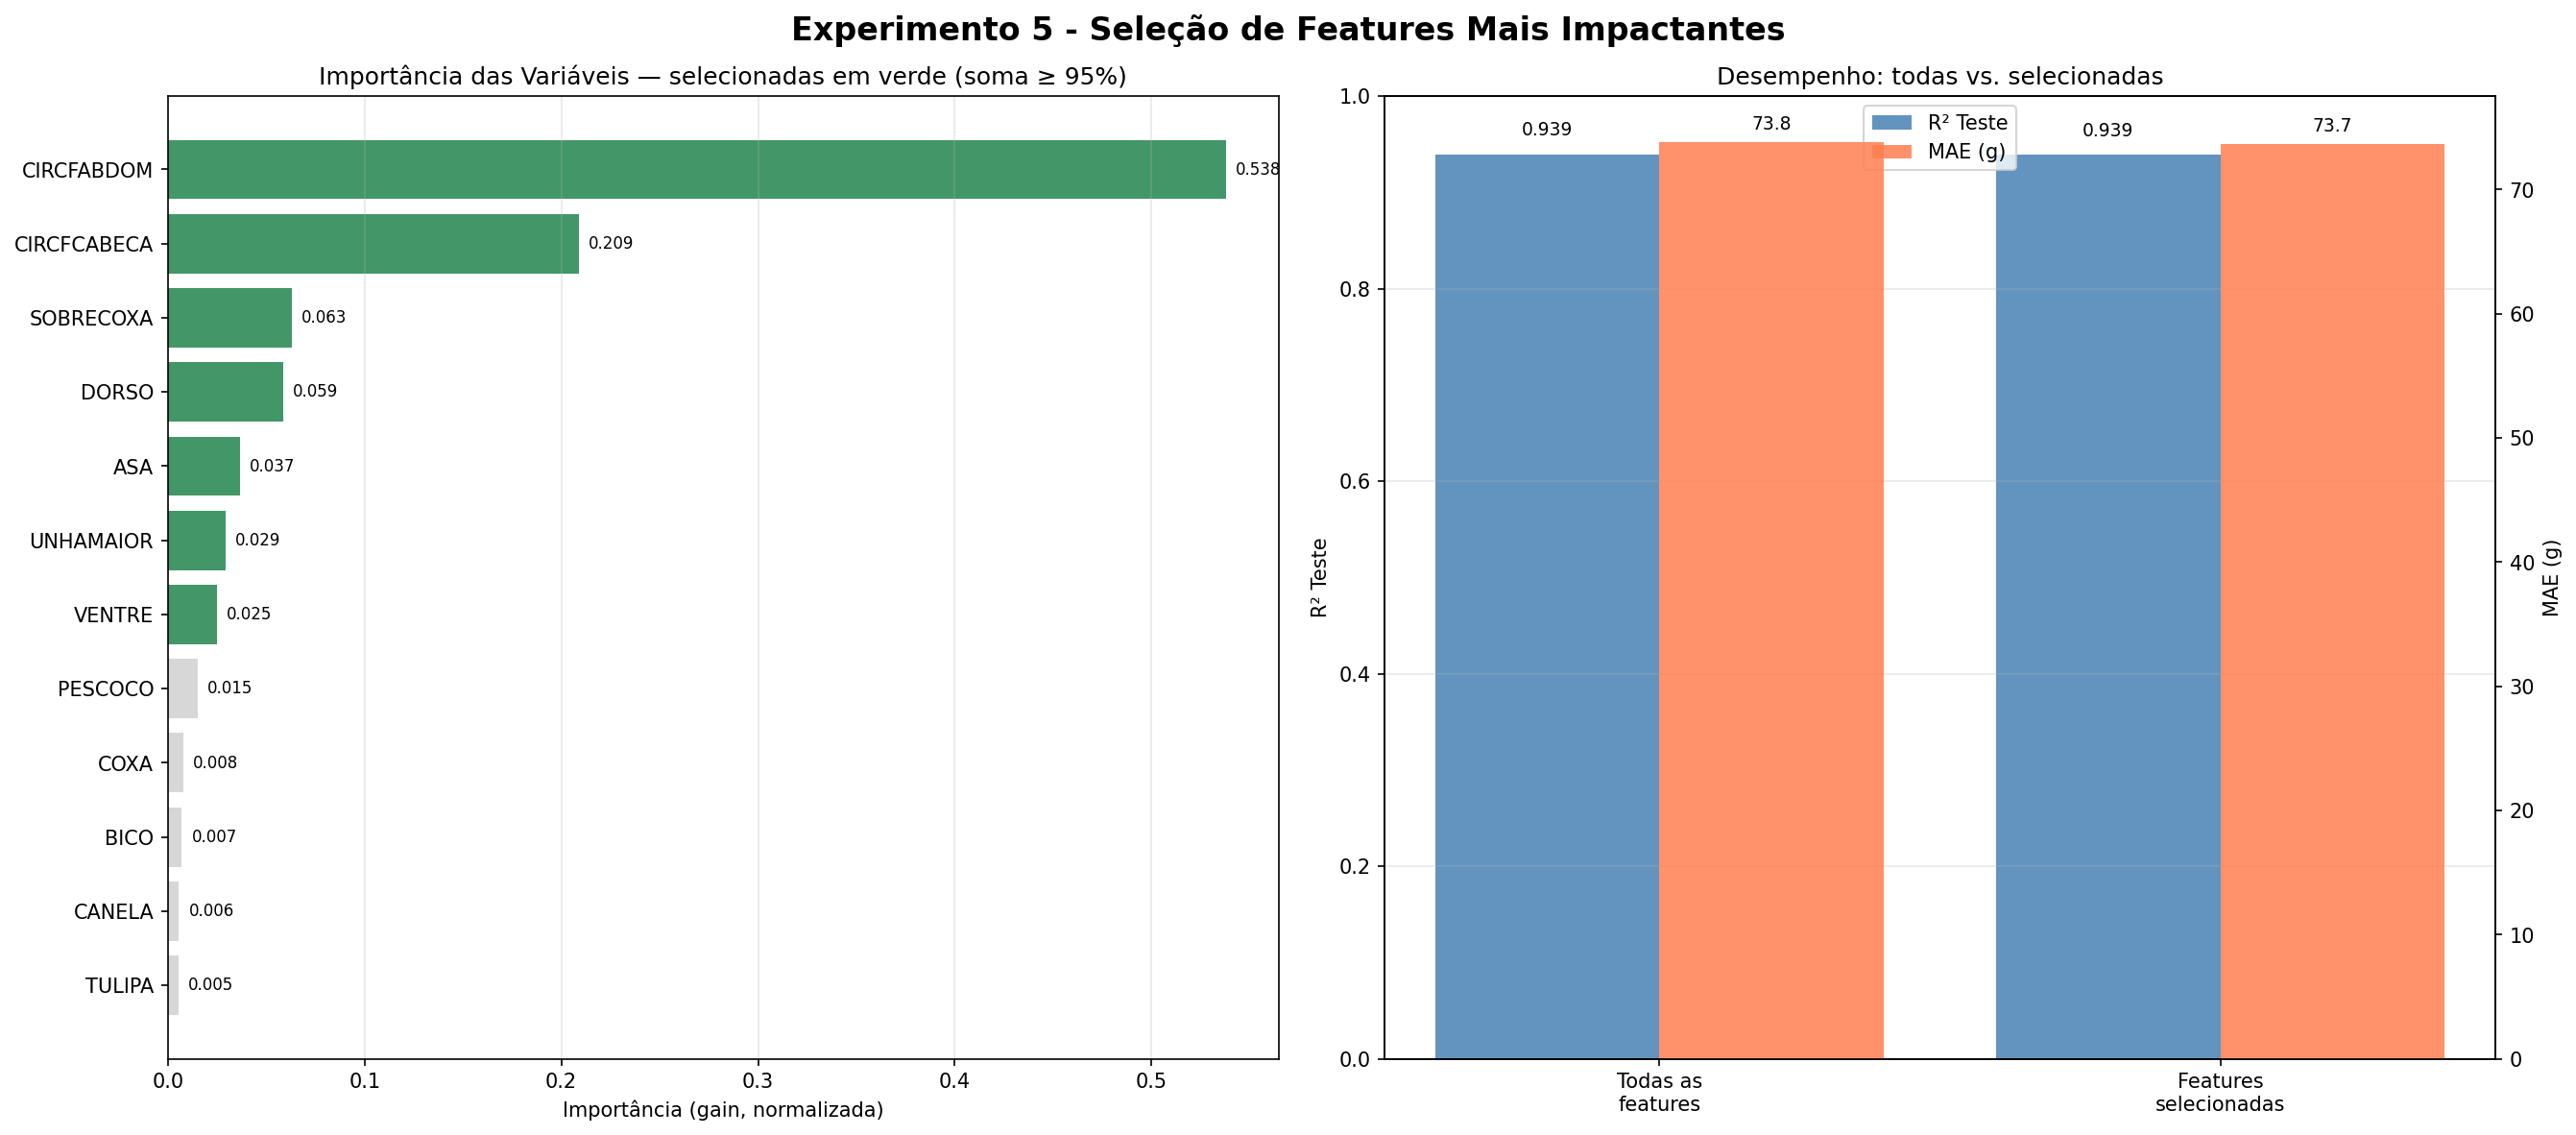
\includegraphics[width=\textwidth]{assets/fig10.png}
\caption{Experimento 5: seleção das variáveis. (A) Importância por ganho de cada medida, com as sete escolhidas em verde. (B) R² de teste e MAE do modelo com todas as variáveis \textit{versus} apenas as selecionadas.}
\label{fig:exp5-features}
\end{figure}

\subsubsection{Desempenho geral e por faixa etária}

Mesmo sem ter acesso à idade das aves, o modelo final obteve R²$_\text{teste}$ = 0,9388, RMSE = 113,3 g e MAE = 73,7 g, o que representa 13,1\% do peso médio no grupo de teste. Esses números são praticamente iguais aos do Experimento 2 (R² = 0,9410) e bem próximos ao melhor modelo do Experimento 3 (R² = 0,9453), mostrando que o resultado geral não depende do algoritmo, do uso da idade ou da quantidade de medidas utilizadas.

A análise detalhada por faixa etária, no entanto, mostra um cenário bem diferente (Tabela~\ref{tab:exp5-idade}).

\begin{table}[htbp]
\centering
\caption{Experimento 5: desempenho dentro de cada faixa etária no grupo de teste.}
\label{tab:exp5-idade}
\begin{tabular}{rrrr}
\hline
\textbf{Idade (dias)} & \textbf{N} & \textbf{R²} & \textbf{MAE (g)} \\
\hline
0 & 47 & $-5,0552$ &  11,6 \\
7 & 47 & $-1,8804$ &  13,1 \\
14 & 48 & $-0,8536$ &  30,3 \\
21 & 46 & $-0,5475$ &  62,9 \\
28 & 47 & $-0,7781$ &  82,7 \\
38 & 47 & $0,5175$ &  65,3 \\
52 & 45 & $0,5062$ &  84,0 \\
66 & 46 & $0,1855$ & 121,4 \\
80 & 43 & $0,2250$ & 125,4 \\
101 & 25 & $-0,3943$ & 175,8 \\
115 & 26 & $0,0341$ & 107,6 \\
\hline
\textbf{Média} & \textemdash & $\mathbf{-0,7310}$ & \textemdash \\
\hline
\end{tabular}
\end{table}

A média do R² dentro de cada idade foi de $-0,731$, o que significa que, para aves com a mesma idade, o modelo erra mais do que se usássemos apenas a média do grupo para prever o peso. Isso aconteceu em cinco das onze idades analisadas, e apenas aos 38 e 52 dias o valor ficou acima de R² = 0,5.

A diferença em relação ao R² geral de 0,9388 só parece contraditória. Na prática, o modelo aprende muito bem a relação entre o tamanho e o peso durante o crescimento, já que separar um filhote de 40 g de uma ave adulta de 1.500 g é algo simples, e essa grande diferença entre as idades é o que puxa o R² geral para cima. O ponto fraco do modelo é diferenciar aves que estão na mesma fase de vida. Vale destacar que tirar a variável IDADE não resolveu esse problema, porque as medidas do corpo aumentam conforme a ave cresce e acabam servindo como um indicativo indireto da idade.

\begin{figure}[htbp]
\centering
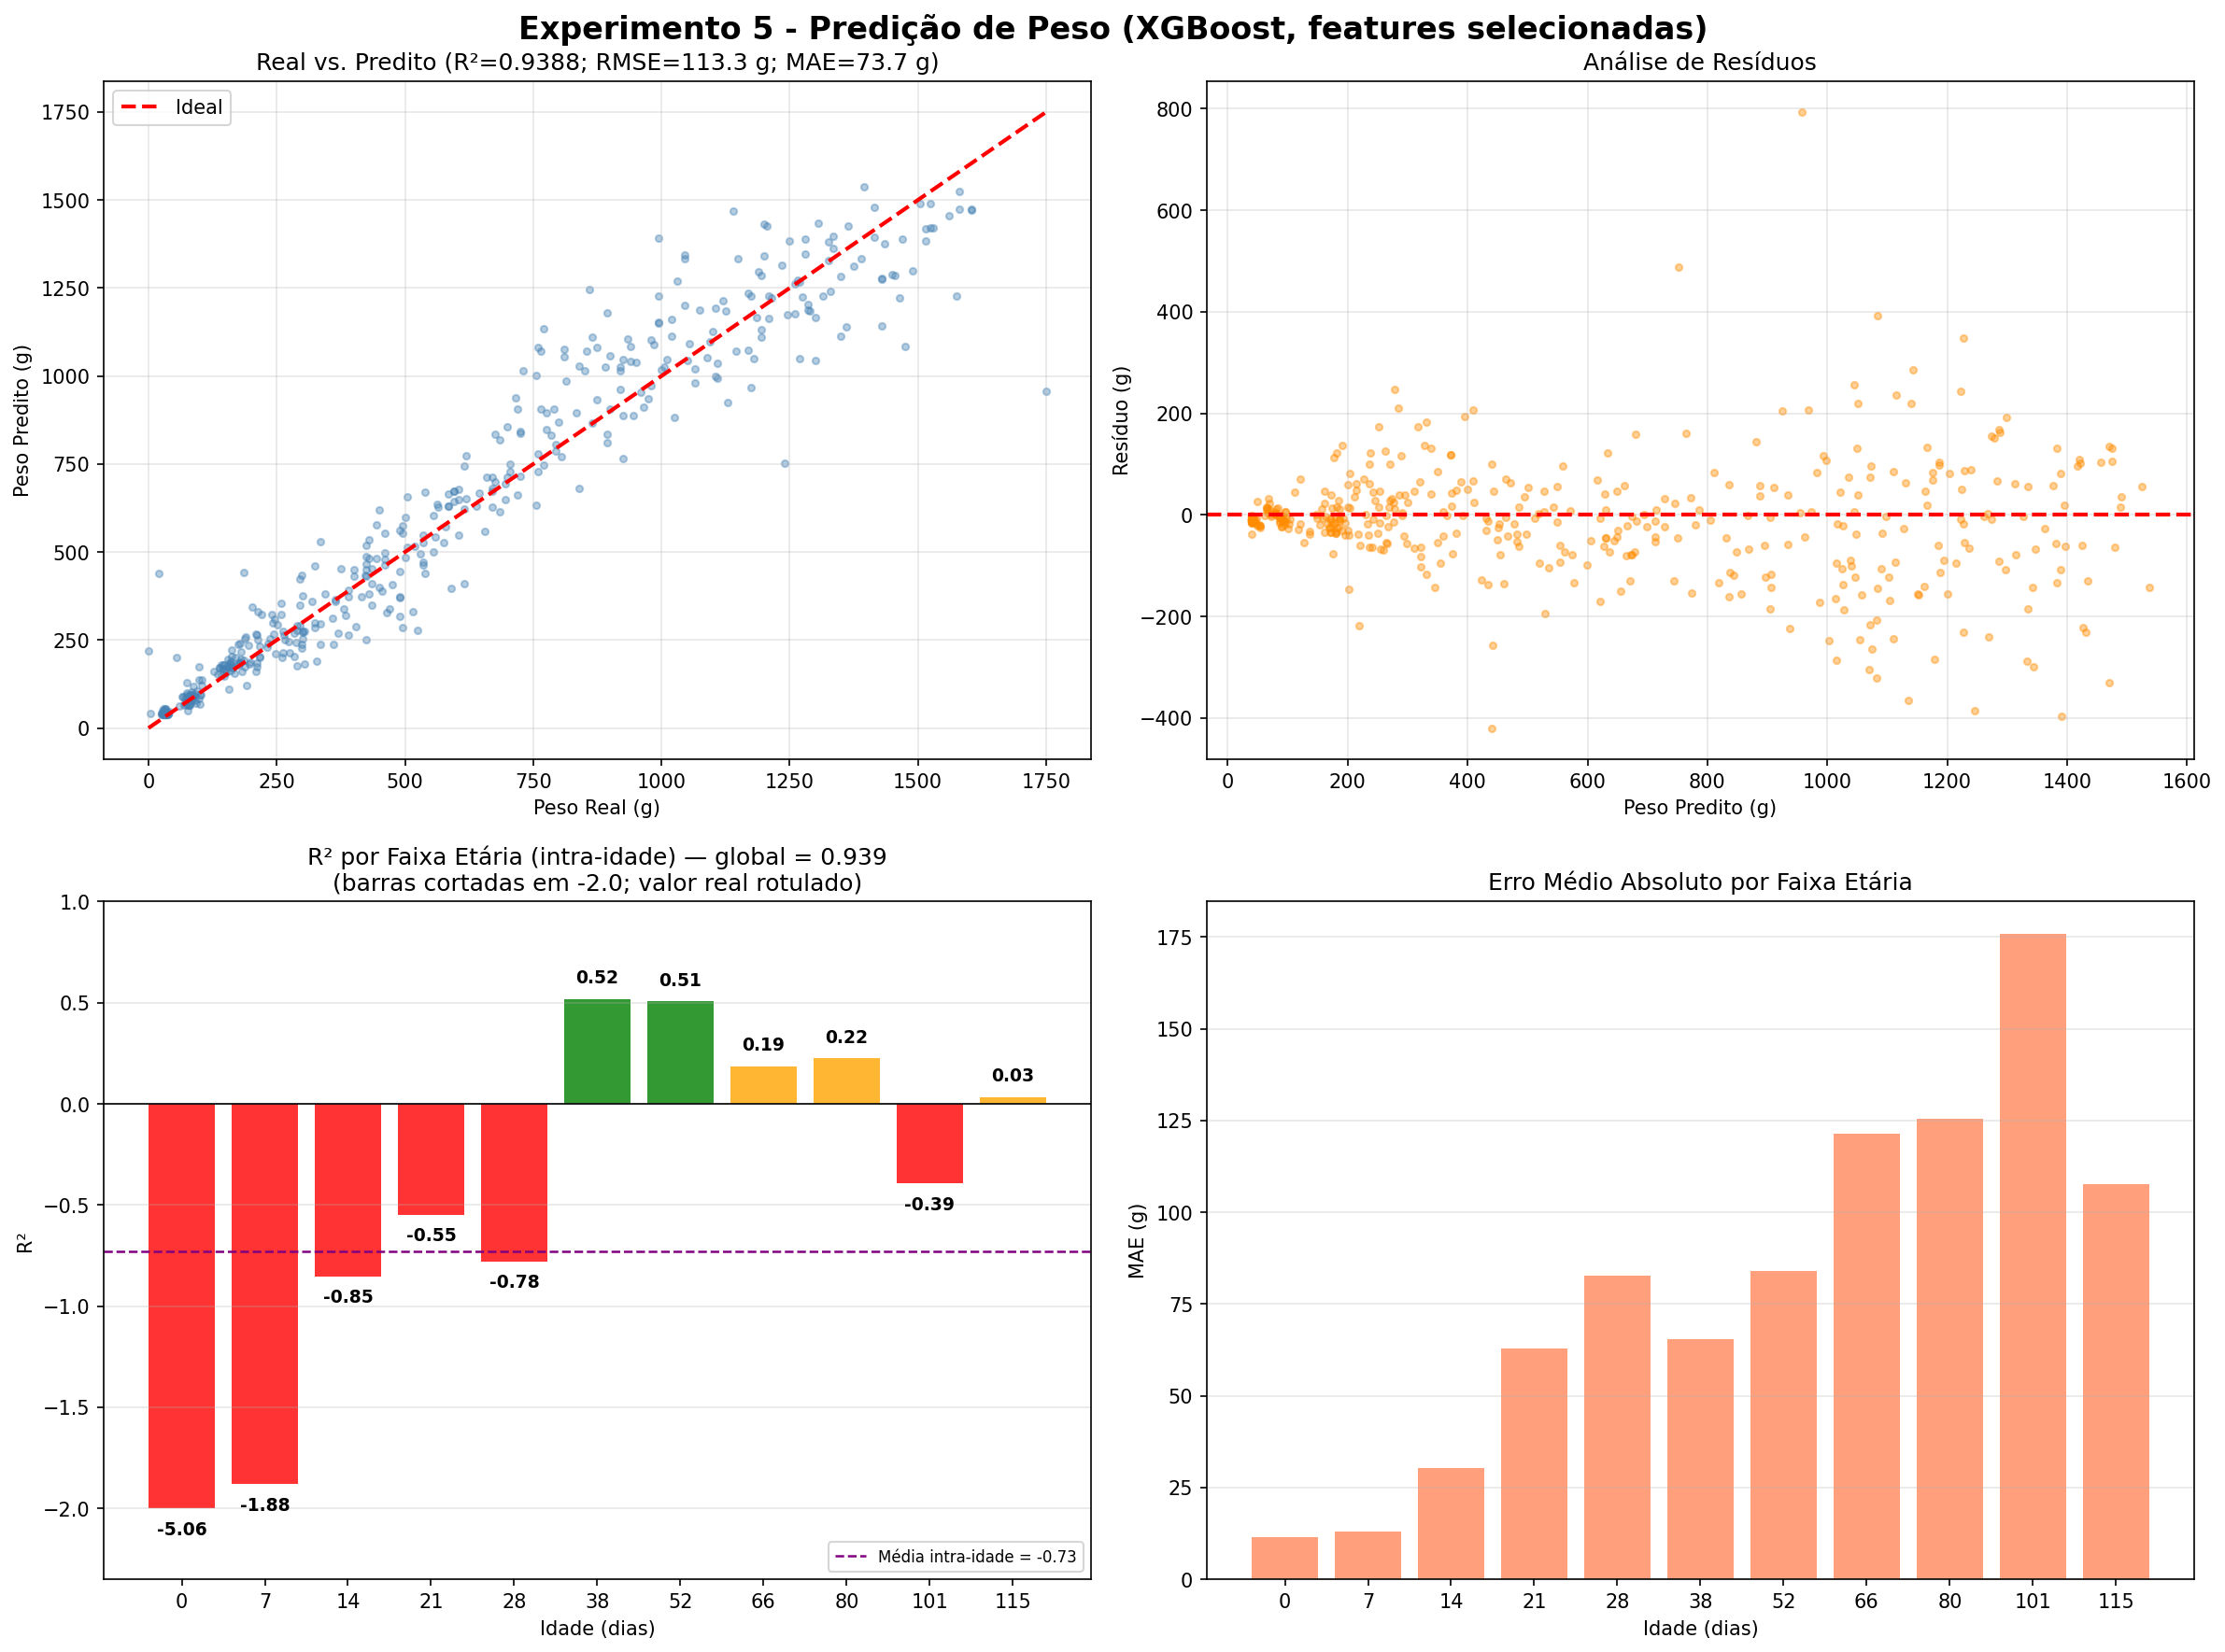
\includegraphics[width=\textwidth]{assets/fig11.png}
\caption{Experimento 5: desempenho do \textit{XGBoost} com as variáveis escolhidas. (A) Valores reais \textit{vs.} previstos. (B) Análise de resíduos. (C) R² dentro de cada faixa etária. (D) Erro médio absoluto por faixa etária.}
\label{fig:exp5-peso}
\end{figure}

\subsubsection{Considerações do Experimento 5}

O experimento traz dois pontos principais. Na prática, apenas sete das doze medidas são suficientes para manter a mesma qualidade do modelo completo, e duas delas concentram cerca de 75\% da importância, o que torna a coleta de medidas no campo mais simples e rápida.

Em termos de metodologia, o R² geral elevado, visto desde o Experimento 1 e comum em outros trabalhos da área, não prova que o modelo é bom para prever o peso de cada animal sozinho, já que ele mede principalmente a curva de crescimento das aves. Ao testar o modelo apenas com aves da mesma idade, que é a situação real de uso em um lote conhecido, os resultados são ruins em média. O modelo serve para estimar o peso esperado para uma fase de crescimento, mas não consegue diferenciar os pesos individuais dentro de um mesmo lote. Por isso, reforça-se a recomendação, já feita no Experimento 3, de usar a análise separada por idade como padrão para apresentar os resultados.


\subsection{Experimento 6}

Os testes anteriores apresentaram resultados fracos e instáveis na hora de identificar o sexo das aves, mas sempre avaliando apenas a saída dos modelos. O Experimento 6 muda o foco da análise: em vez de testar diferentes classificadores, busca entender se existe alguma informação sobre o sexo nas medidas do corpo, partindo direto dos dados brutos até chegar ao algoritmo. Foram reunidas cinco evidências distintas, cobrindo distribuições por sexo, testes de dimorfismo por faixa etária, projeções de várias medidas juntas, importância das variáveis e curva ROC.

\subsubsection{Distribuição das medidas por sexo}

Analisando os 2.299 registros, as distribuições de machos e fêmeas são praticamente iguais. No peso corporal (Figura~\ref{fig:exp6-box-peso}), o valor do meio (mediana) para os machos foi de 475,0 g contra 460,0 g para as fêmeas, o que representa uma diferença de apenas 3,3\%, valor sem impacto prático diante da variação geral dos dois grupos, que vai de cerca de 160 g a 1.000 g.

O cálculo da correlação entre cada medida e o sexo confirma essa semelhança: todos os catorze valores ficaram entre $-0,004$ (BICO) e $+0,043$ (CANELA). O único resultado estatisticamente significativo a 5\% foi o da canela ($r = +0,043$; $p = 0,038$), mas um número tão baixo explica menos de 0,2\% da variação do sexo. A Figura~\ref{fig:exp6-box-canela} destaca essa medida, que foi a mais informativa de todas: a mediana ficou em 5,0 cm para machos e 4,8 cm para fêmeas, gerando caixas quase sobrepostas no gráfico.

\begin{figure}[htbp]
\centering
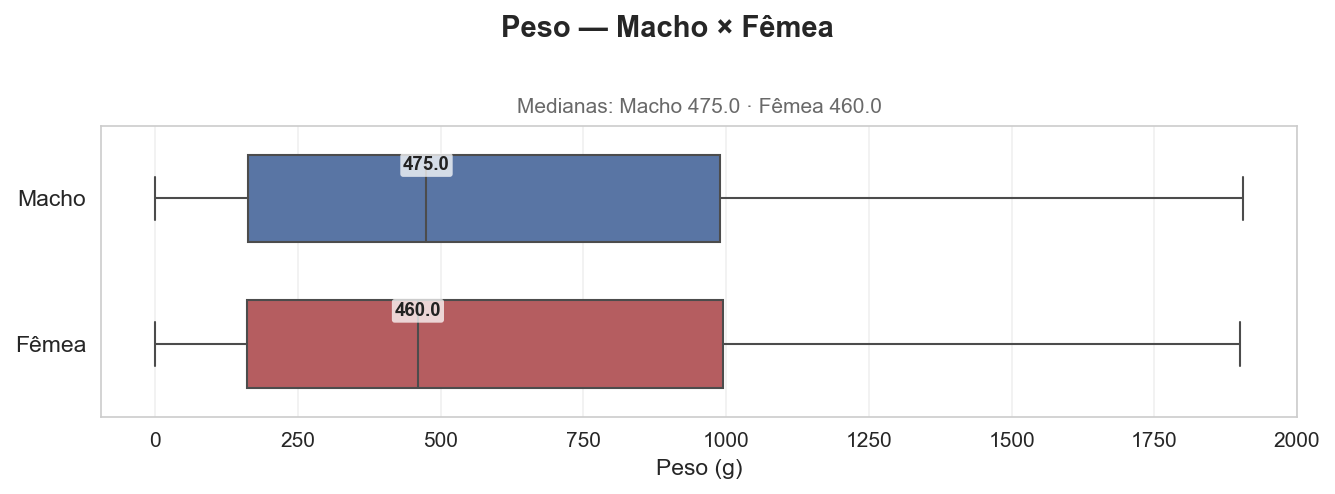
\includegraphics[width=\textwidth]{assets/fig12.png}
\caption{Distribuição do peso corporal por sexo, considerando todas as idades.}
\label{fig:exp6-box-peso}
\end{figure}

\begin{figure}[htbp]
\centering
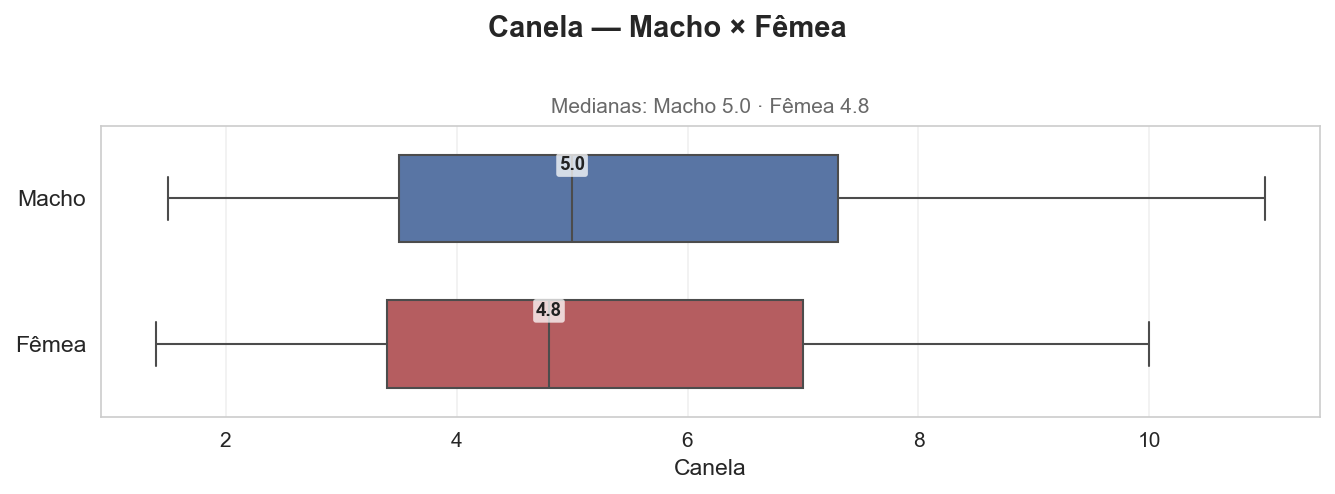
\includegraphics[width=\textwidth]{assets/fig13.png}
\caption{Distribuição do comprimento da canela por sexo, sendo esta a variável com maior relação com o sexo em todo o conjunto.}
\label{fig:exp6-box-canela}
\end{figure}

\subsubsection{Diferença entre sexos por faixa etária}

Um ponto a se considerar é que as diferenças físicas poderiam aparecer apenas em certas idades e acabar sumindo na análise geral. A Tabela~\ref{tab:exp6-dimorfismo} analisa essa possibilidade comparando a média de peso de machos e fêmeas em cada uma das onze idades, por meio do teste de Mann-Whitney.

\begin{table}[htbp]
\centering
\footnotesize
\caption{Diferença de peso entre machos e fêmeas por faixa etária (teste de Mann-Whitney).}
\label{tab:exp6-dimorfismo}
\begin{tabular}{rrrrrc}
\hline
\textbf{Idade (dias)} & \textbf{Machos (g)} & \textbf{Fêmeas (g)} &
\textbf{Diferença (\%)} & \textbf{$p$-valor} & \textbf{Significativo?} \\
\hline
0 &   32,1 &   32,2 & $-0,3$ & 0,9327 & não \\
7 &   84,0 &   81,8 & $+2,8$ & 0,1275 & não \\
14 &  167,3 &  170,7 & $-2,0$ & 0,2098 & não \\
21 &  266,3 &  249,7 & $+6,7$ & 0,0666 & não \\
28 &  410,0 &  389,7 & $+5,2$ & 0,0973 & não \\
38 &  573,8 &  554,8 & $+3,4$ & 0,1901 & não \\
52 &  800,6 &  784,5 & $+2,0$ & 0,3534 & não \\
66 &  987,9 &  970,2 & $+1,8$ & 0,5626 & não \\
80 & 1157,0 & 1180,8 & $-2,0$ & 0,4413 & não \\
101 & 1264,4 & 1286,1 & $-1,7$ & 0,4832 & não \\
115 & 1434,3 & 1430,6 & $+0,3$ & 0,9162 & não \\
\hline
\end{tabular}
\end{table}

Em nenhuma das onze idades houve diferença estatisticamente significativa. As variações percentuais foram de $-2,0\%$ a $+6,7\%$ e não mantiveram um padrão fixo, já que em quatro idades as fêmeas foram, em média, mais pesadas que os machos.

O mesmo teste aplicado para cada medida corporal dentro de cada idade gerou 77 comparações, das quais 14 tiveram $p < 0,05$. O total ficou um pouco acima dos quatro casos esperados ao acaso, mas essas diferenças apareceram espalhadas entre idades e medidas sem uma regra clara, e nenhuma se manteve válida após o ajuste de Bonferroni para testes múltiplos (limite de 0,00065, sendo que o menor valor encontrado foi $p = 0,00074$, para a coxa aos 66 dias). A Figura~\ref{fig:exp6-separabilidade} resume essa situação: mesmo combinando as duas medidas mais fortes de cada idade, machos e fêmeas continuam totalmente misturados no gráfico.

\begin{figure}[htbp]
\centering
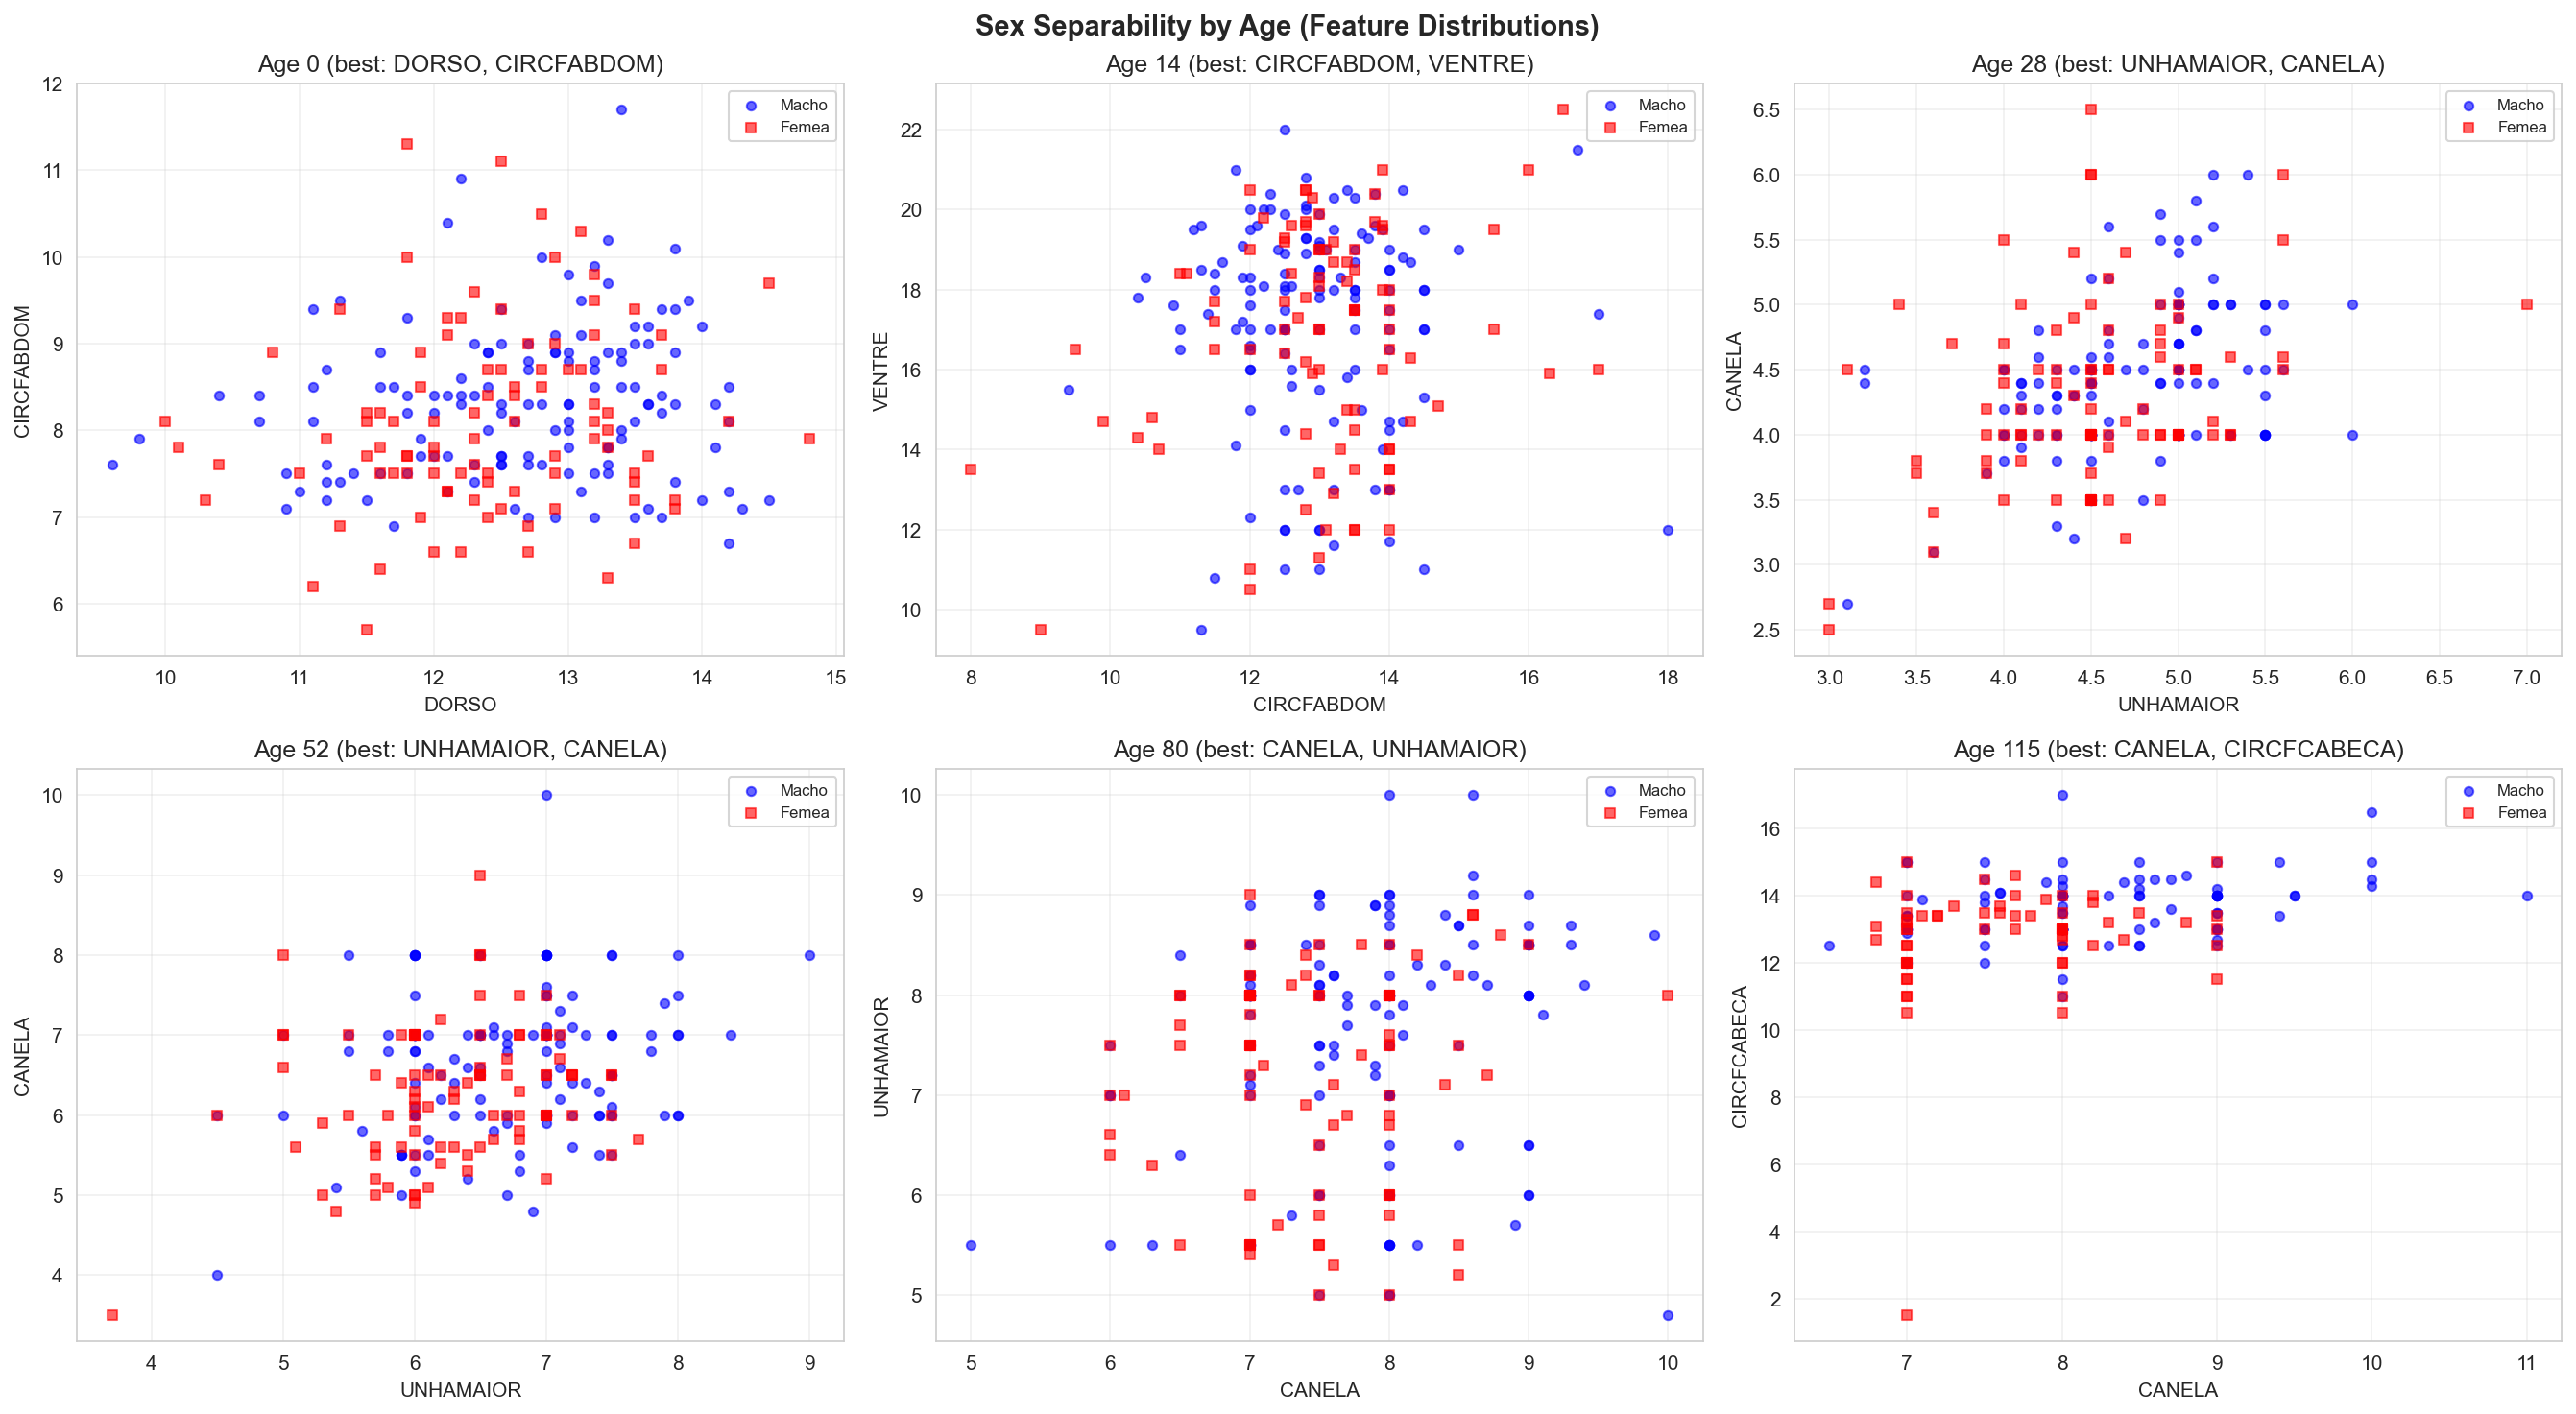
\includegraphics[width=\textwidth]{assets/fig14.png}
\caption{Separação dos sexos por faixa etária. Cada gráfico mostra o cruzamento das duas variáveis com menor $p$-valor naquela idade.}
\label{fig:exp6-separabilidade}
\end{figure}

\subsubsection{Combinação de múltiplas variáveis}

As etapas anteriores avaliaram as medidas uma a uma. No entanto, é possível que a separação entre os sexos só fique visível ao combinar várias características ao mesmo tempo. Para verificar isso, foram usadas duas técnicas de projeção.

A análise de componentes principais (Figura~\ref{fig:exp6-pca}) mostra que o primeiro eixo concentra 83,2\% de toda a variação dos dados e reflete simplesmente o tamanho geral da ave, ou seja, a sua idade; o segundo eixo explica apenas 3,7\%. Com isso, machos e fêmeas ocupam o mesmo espaço no gráfico.

A análise discriminante linear (Figura~\ref{fig:exp6-lda}) reforça esse ponto, pois é um método feito justamente para tentar encontrar a melhor combinação para separar os dois grupos. Mesmo assim, as curvas de machos e fêmeas ficaram quase sobrepostas, mudando apenas por um leve desvio nas médias.

\begin{figure}[htbp]
\centering
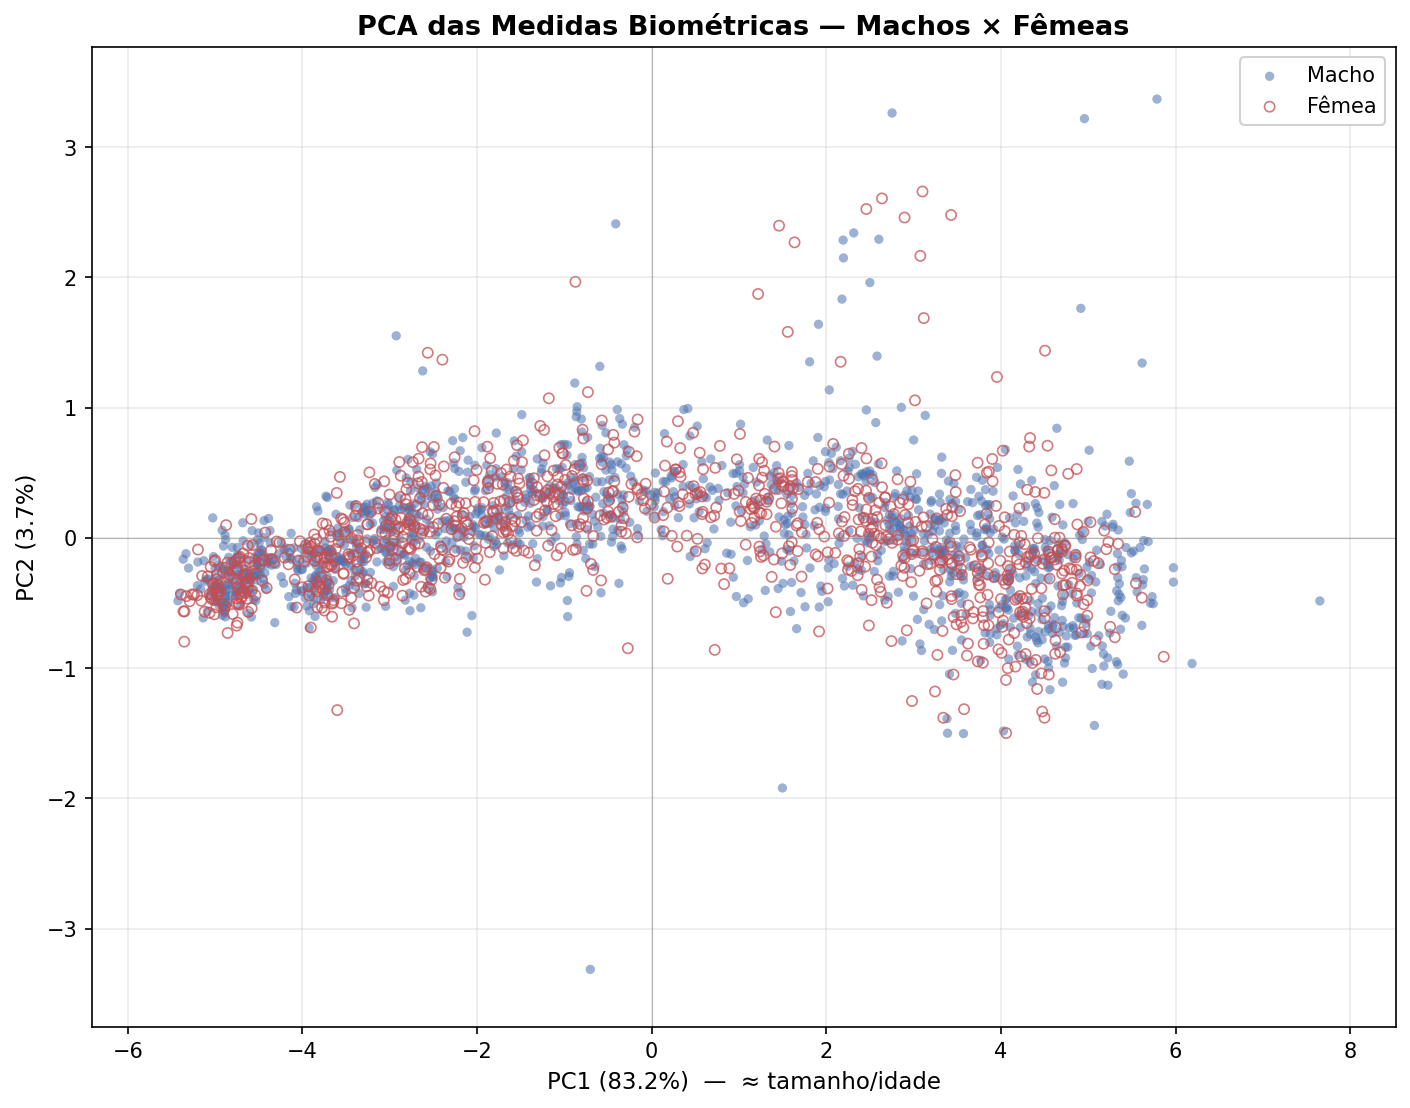
\includegraphics[width=0.85\textwidth]{assets/fig15.png}
\caption{Projeção das medidas corporais nos dois eixos principais, com as aves divididas por sexo.}
\label{fig:exp6-pca}
\end{figure}

\begin{figure}[htbp]
\centering
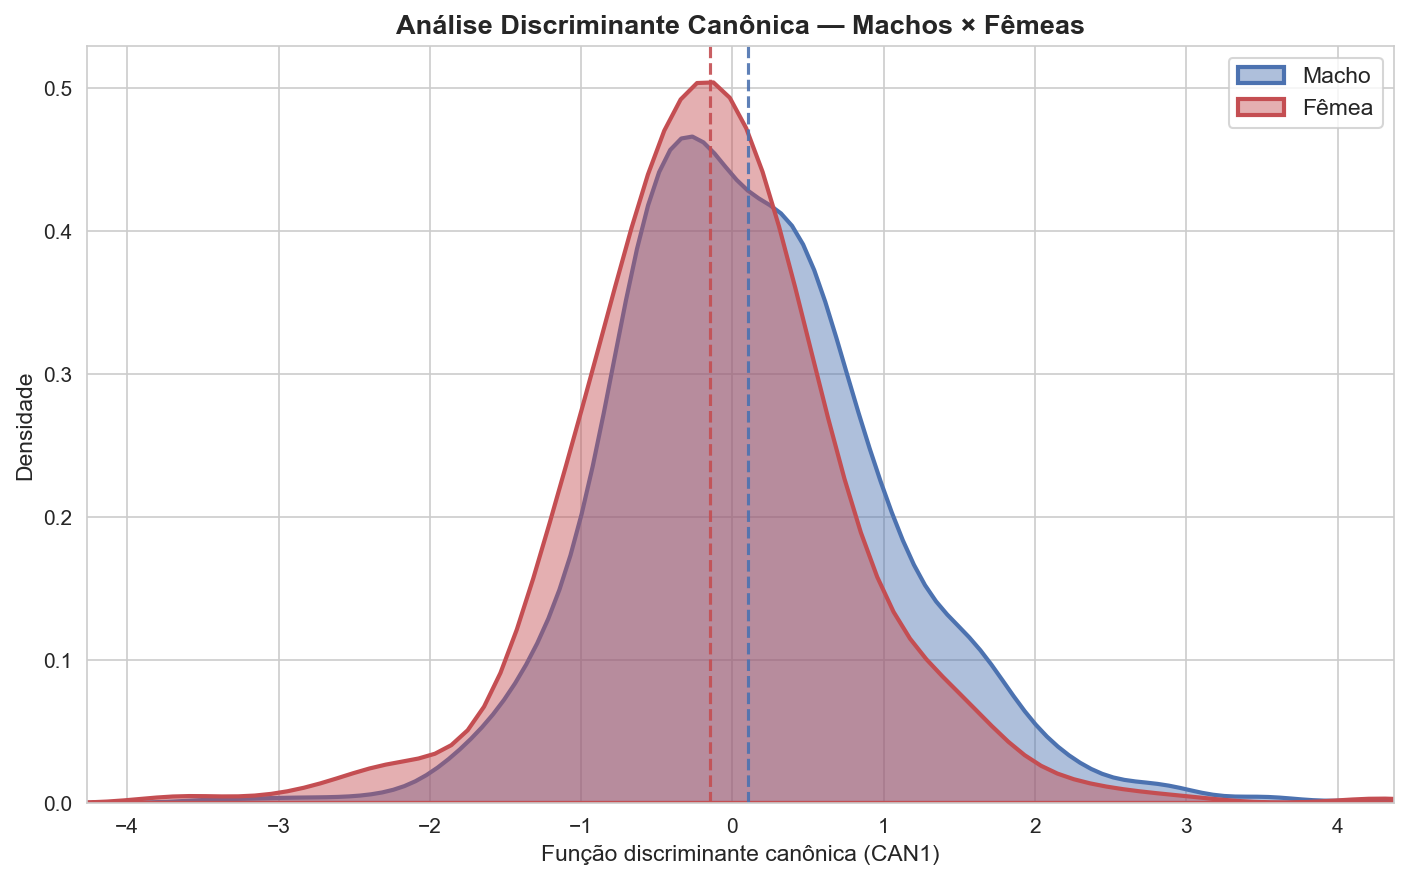
\includegraphics[width=0.85\textwidth]{assets/fig16.png}
\caption{Distribuição de machos e fêmeas ao longo da função de separação dos grupos.}
\label{fig:exp6-lda}
\end{figure}

\subsubsection{Capacidade de classificação do modelo}

Por fim, ajustou-se um modelo \textit{XGBoost Classifier} usando as treze medidas corporais junto com o peso e a idade. A importância de cada variável no modelo (Figura~\ref{fig:exp6-importancia}) ficou dividida de forma quase igual, variando entre 0,064 e 0,092, faixa bem próxima dos 0,071 esperados caso o peso fosse distribuído igualmente entre as catorze variáveis. Nenhuma característica se destacou para a divisão dos grupos, o que acontece quando os dados não trazem nenhum padrão claro.

A curva ROC (Figura~\ref{fig:exp6-roc}) mostra os limites desse modelo: o resultado de AUC foi de 0,602 no grupo de teste e 0,565 na validação cruzada, com acerto geral (acurácia) de 0,557. Como uma escolha totalmente aleatória gera uma AUC de 0,500, o ganho real do modelo sobre a sorte foi de apenas 0,10, valor insuficiente para qualquer uso prático.

\begin{figure}[htbp]
\centering
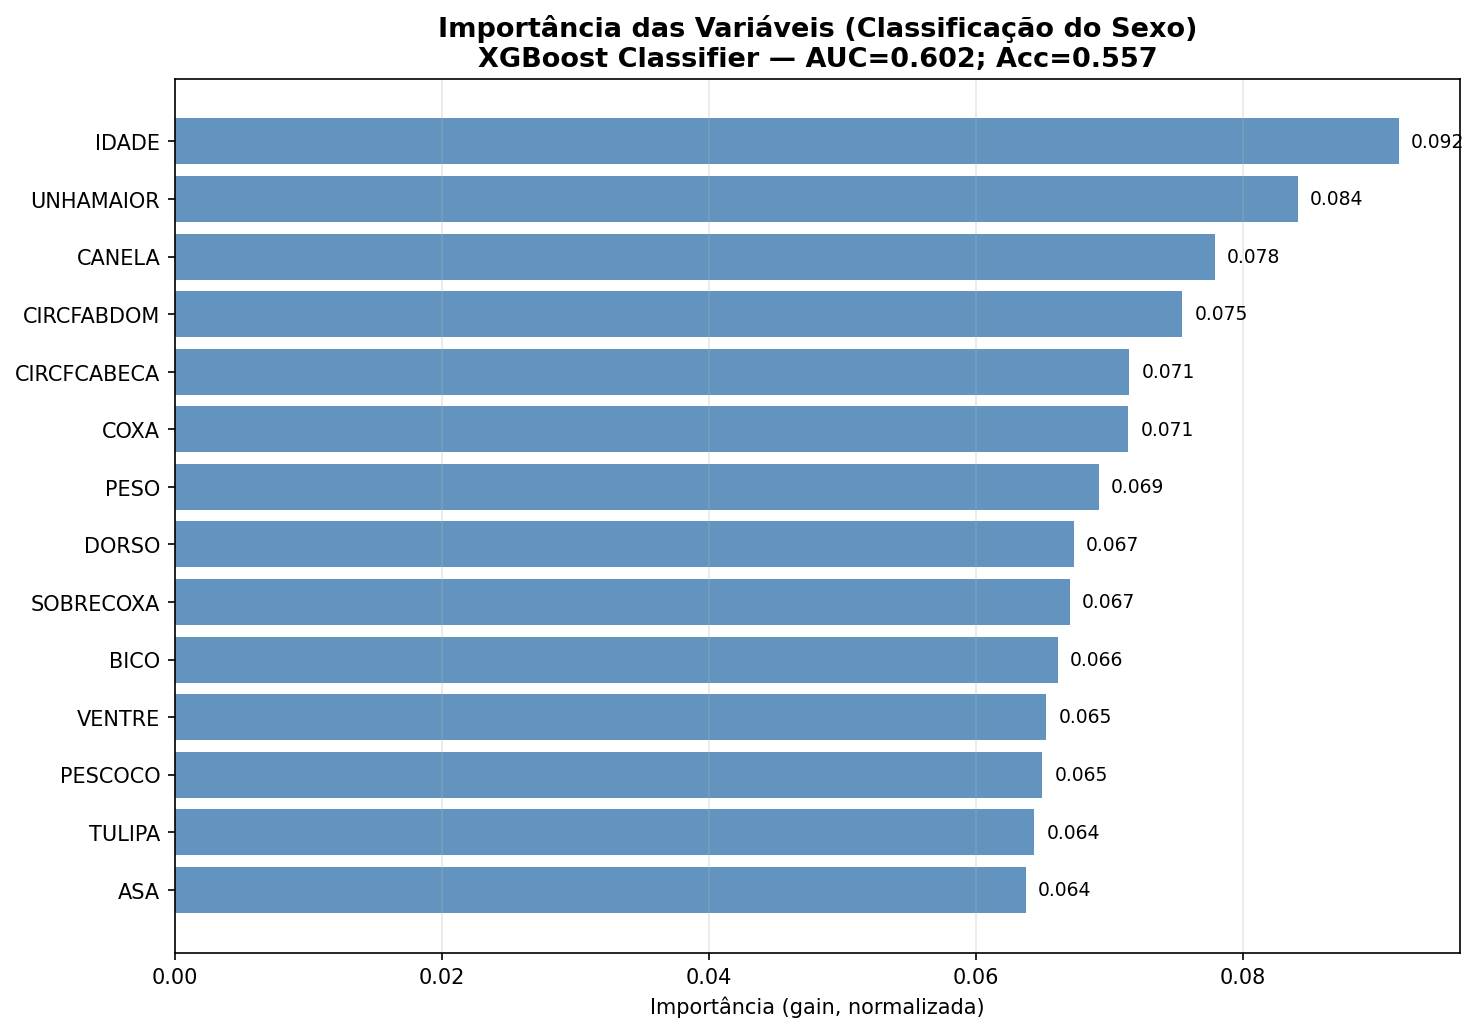
\includegraphics[width=0.9\textwidth]{assets/fig17.png}
\caption{Importância de cada variável no modelo \textit{XGBoost Classifier} para identificar o sexo.}
\label{fig:exp6-importancia}
\end{figure}

\begin{figure}[htbp]
\centering
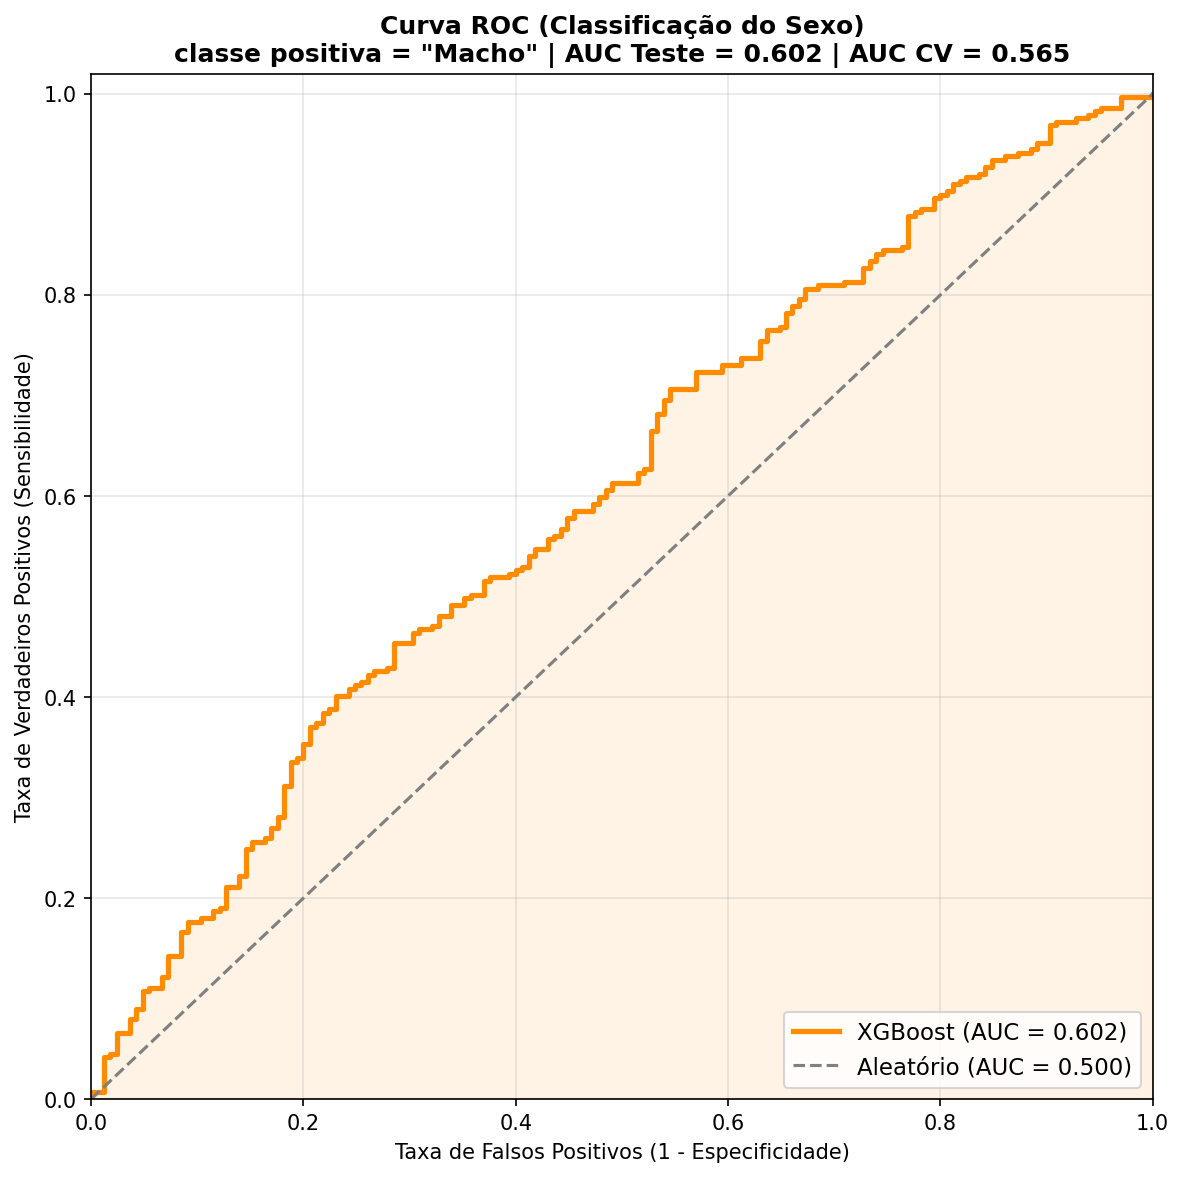
\includegraphics[width=0.7\textwidth]{assets/fig18.png}
\caption{Curva ROC para a identificação do sexo, considerando a classe "Macho" como positiva.}
\label{fig:exp6-roc}
\end{figure}

\subsubsection{Considerações do Experimento 6}

Os cinco testes trazem a mesma resposta: os dados de machos e fêmeas se sobrepõem, nenhuma idade traz diferenças físicas claras, a união de várias variáveis não separa os grupos, o peso de cada medida no modelo é quase igual e a taxa de acerto fica próxima da escolha ao acaso. Essas constatações vêm de cinco etapas independentes, desde a análise direta das medidas até a avaliação do modelo final.

Dessa forma, fica claro que o desempenho baixo nos Experimentos 1 a 4 não aconteceu por escolha errada de algoritmo, desequilíbrio na base ou falta de ajuste nos parâmetros: a resposta simplesmente não está nas medidas corporais. Para as medidas avaliadas, a galinha-d'angola se comporta como uma espécie sem diferenças visíveis entre os sexos, o que concorda com Vieira et al. (2009), que indicam a falta de dimorfismo evidente em pelo menos metade das espécies de aves.

Na prática, isso define o limite da proposta: prever o peso usando medidas do corpo é um caminho viável, mas separar os sexos dessa forma não funciona. Para identificar o sexo, seria necessário recorrer a outros tipos de dados, como o som emitido pelas aves, detalhes nas penas ou testes genéticos.

\section{Conclusão}

Este trabalho apresentou a aplicação de técnicas de aprendizado de máquina para
a predição do peso corporal e classificação do sexo de galinhas-d'angola a
partir de medidas morfométricas.

Os resultados indicaram que o modelo \textit{XGBoost} possui elevada capacidade
preditiva para o peso corporal, especialmente quando há utilização de variáveis
historicamente correlacionadas, como o PESO\_ANTERIOR. No entanto, verificou-se
que essa dependência pode inflar artificialmente o desempenho, reduzindo a
interpretabilidade e a capacidade de generalização do modelo. No Experimento 2, ao
utilizar um modelo unificado sem essa dependência explícita, observou-se uma
leve redução no desempenho, porém com maior robustez e coerência metodológica.

Para a classificação do sexo, os modelos avaliados apresentaram desempenho
limitado e inconsistente entre as diferentes idades. Mesmo os melhores
algoritmos demonstraram viés significativo na classificação, com maior acurácia
para machos e dificuldade na identificação de fêmeas. Esses resultados sugerem
que as medidas morfométricas utilizadas não são suficientemente discriminativas
para essa tarefa em todas as fases de desenvolvimento.

De forma geral, os experimentos mostram um compromisso entre desempenho e
capacidade de generalização, destacando a importância da seleção adequada de
variáveis e da análise crítica dos resultados. Como perspectivas futuras,
propõe-se a investigação de novas variáveis, técnicas de balanceamento de dados
e a avaliação de modelos mais robustos, visando aprimorar a confiabilidade das
predições.

Os resultados evidenciam o potencial do uso de aprendizado de máquina na
avicultura, ao mesmo tempo em que destacam limitações importantes relacionadas
à qualidade e natureza dos dados, reforçando a necessidade de abordagens
híbridas e novos tipos de variáveis.

\section*{Referências}
\nocite{*}
\bibliographystyle{sbc}
\bibliography{sbc-template}

\end{document}
